% ------------------------------------------------------------------------
% ------------------------------------------------------------------------
% ICMC: Modelo de Trabalho Acadêmico (tese de doutorado, dissertação de
% mestrado e trabalhos monográficos em geral) em conformidade com
% ABNT NBR 14724:2011: Informação e documentação - Trabalhos acadêmicos -
% Apresentação
% ------------------------------------------------------------------------
% ------------------------------------------------------------------------

% Opções:
%   Qualificação          = qualificacao
%   Curso                 = doutorado/mestrado
%   Situação do trabalho  = pre-defesa/pos-defesa (exceto para qualificação)
%   Versão para impressão = impressao
\documentclass[mestrado, pre-defesa, draft]{packages/icmc}

% ---------------------------------------------------------------------------
% Pacotes Opcionais
% ---------------------------------------------------------------------------
\usepackage{rotating}           % Usado para rotacionar o texto
\usepackage[all,knot,arc,import,poly]{xy}   % Pacote para desenhos gráficos
% Este pacote pode conflitar com outros pacotes gráficos como o ``pictex''
% Então é necessário usar apenas um dos pacotes conflitantes
\newcommand{\VerbL}{0.52\textwidth}
\newcommand{\LatL}{0.42\textwidth}
% ---------------------------------------------------------------------------


% ---
% Informações de dados para CAPA e FOLHA DE ROSTO
% ---
% Tanto na capa quanto nas folhas de rosto apenas a primeira letra da primeira palavra (ou nomes próprios) devem estar em letra maiúscula, todas as demais devem ser em letra minúscula.
\tituloPT{Geradores de homologia persistente e aplicações}
\tituloEN{Persistent homology generators and applications}
\autor[Ronchi, C. H. V.]{Carlos Henrique Venturi Ronchi}
\genero{M} % Gênero do autor (M = Masculino / F = Feminino)
\orientador[Orientador]{Prof. Dr.}{Marcio Fuzeto Gameiro}
\curso{MAT}
\data{10}{2019} % Data do depósito
\idioma{PT} % Idioma principal do documento (PT = português / EN = inglês)
% ---

% include necessary packages
\usepackage{packages/carlos_package}

% ---
% RESUMOS
% ---

% Resumo em PORTUGUÊS
% conter no máximo 500 palavras
% conter no mínimo 1 e no máximo 5 palavras-chave
\textoresumo[brazil]{
    a.
    }{Modelo, Monografia de qualificação, Dissertação, Tese, Latex}


% resumo em INGLÊS
% conter no máximo 500 palavras
% conter no mínimo 1 e no máximo 5 palavras-chave
\textoresumo[english]{
    a.
    }{Template, Qualification monograph, Dissertation, Thesis, Latex}


% ----------------------------------------------------------
% ELEMENTOS PRÉ-TEXTUAIS
% ----------------------------------------------------------

% Inserir a ficha catalográfica
\incluifichacatalografica{tex/pre-textual/ficha-catalografica.pdf}

% DEDICATÓRIA / AGRADECIMENTO / EPÍGRAFE
%\textodedicatoria*{tex/pre-textual/dedicatoria}
%\textoagradecimentos*{tex/pre-textual/agradecimentos}
%\textoepigrafe*{tex/pre-textual/epigrafe}

% Inclui a lista de figuras
\incluilistadefiguras

% Inclui a lista de tabelas
\incluilistadetabelas

% Inclui a lista de quadros
%\incluilistadequadros

% Inclui a lista de algoritmos
\incluilistadealgoritmos

% Inclui a lista de códigos
\incluilistadecodigos

% Inclui a lista de siglas e abreviaturas
%\incluilistadesiglas

% Inclui a lista de símbolos
%\incluilistadesimbolos

% ----
% Início do documento
% ----
\begin{document}
% ----------------------------------------------------------
% ELEMENTOS TEXTUAIS
% ----------------------------------------------------------
\textual

\chapter{Introdução}
\label{chapter:introducao}
% Comando simples para exibir comandos Latex no texto
\newcommand{\comando}[1]{\textbf{$\backslash$#1}}

Este documento explica brevemente como trabalhar com a classe \LaTeX~\textit{icmc} para confeccionar trabalhos acadêmicos seguindo as normas da \sigla{ABNT}{Associação Brasileira de Normas Técnicas} e as \aspas{\textit{Diretrizes para apresentação de dissertações e teses da USP: documento eletrônico e impresso. Parte I (ABNT)}}, publicado pelo \sigla{SIBi}{Sistema Integrado de Bibliotecas} USP. O presente manual também atende as exigências prevista no regimento do Programa de Pós-graduação em \sigla{CCMC}{Ciências da Computação e Matemática Computacional} do \sigla{ICMC}{Instituto de Ciências Matemáticas e de Computação} da \sigla{USP}{Universidade de São Paulo}.


A classe \textit{icmc} foi construída com base na última versão da classe \textit{abntex2} e do pacote \textit{abntex2cite}. Portanto, este documento exemplifica a elaboração de trabalho
acadêmico (tese, dissertação e outros do gênero) produzido conforme a ABNT NBR
14724:2011 \textit{Informação e documentação - Trabalhos acadêmicos - Apresentação}.

Assim, é altamente recomendável que seja consultada a documentação do \textit{abntex2}\footnote{http://abntex.net.br}. A classe \textit{abntex2} foi desenvolvida para facilitar a escrita de documentos seguindo as normas da ABNT no ambiente \LaTeX\;\cite{frasson:2005:classe_abnt}.

Todo o trabalho de pesquisa e ajustes da presente classe \LaTeX~\emph{icmc} foram feitos pelo aluno mestrado do Programa de Pós-graduação em Ciência da Computação e Matemática Computacional, Humberto Lidio Antonelli, durante a confecção da sua monografia de qualificação.

O requisito básico para utilização da classe \textit{icmc} é criar um documento desta classe com o comando
\comando{documentclass[@parameters]\{icmc\}} e ter, no diretório de trabalho, o arquivo \emph{icmc.cls} presente. Entretanto, recomenda-se fortemente manter a estrutura de diretório inicial fornecida por este modelo. Além disso, para que o documento esteja em conformidade com as normas exigidas pelo programa de Pós-Graduação, o \textbf{projeto deve ser compilado utilizando \textit{XeLaTeX} ou \textit{LuaLaTeX}}. Esse processo de compilação é necessário para que as fontes externas utilizadas para gerar a capa sejam incluídas.

Os parâmetros possíveis utilizados pelo \comando{documentclass} são:
\begin{description}
\item[qualificacao] Exclusivamente para monografias de qualificação em geral;
\item[mestrado / doutorado] Identifica o curso ao qual o aluno pertence, sendo utilizado apenas uma das duas opcões disponíveis. O valor padrão é \textbf{doutorado};
\item[pre-defesa / pos-defesa] Identifica a situação do documento (exceto para qualificação), sedo necessário apenas uma das duas opções. O valor padrão é \textbf{pos-defesa};
\item[impressao] Gera exclusivamente uma versão para impressão do documento;
\item[french, spanish, english, brazil] Adiciona o idioma para correta hifenização correta no documento. Os idiomas bases para o modelo (português e inglês) não precisam ser declarados.
\end{description}


\chapter{Homologia Persistente 101}
\label{chapter:hp101}
A topologia sempre foi vista como uma área de abstração da matemática, sem
espaço para aplicações. Ela é usada para o estudo de diversos espaços
em sua forma abstrata, auxiliando matemáticos em diversas demonstrações
de teoremas e dando uma base fundamental para grande parte da teoria matemática
usada no dia a dia~\cite{Poincare1895}.

Certas propriedades dos espaços topológicos são estudadas através da
topologia algébrica, dando algumas informações, como o número de componentes
conexas por caminhos de um espaço e buracos. A princípio esta é uma área altamente
abstrata da matemática,  nos últimos anos esta visão foi mudando,
com o desenvolvimento da Homologia Persistente e Análise Topológica de Dados.

Um conjunto de dados, geralmente um subconjunto finito de algum espaço métrico,
pode ser estudado através da homologia persistente e assim obtemos informações
topológicas do objeto em estudo.

O pipeline da análise topológica de dados pode ser divido nos seguintes passos:
\begin{itemize}
  \item A entrada do algoritmo pode ser um conjunto de pontos ou alguma matriz
  de distância/similaridade do conjunto de dados.
  \item A construção de um objeto combinatorial em cima do conjunto de dados ou
  da matriz de distância. Geralmente uma filtração ou um complexo simplicial.
  \item A partir da filtração ou do complexo simplicial é possível extrair informações
  topológicas e geométricas do conjunto de dados, por exemplo o número de
  componentes conexas, como um algoritmo de Clustering.
  \item Por fim a interpretação dos dados obtidos e possível pós processamento
  para a utilização em outros algoritmos, como os de classificação ou regressão.
\end{itemize}

Neste capítulo descrevemos de forma ingênua a homologia persistente, começando com
filtrações, passando pelos espaços vetoriais associados
aos complexos simpliciais e chegando ao algoritmo de homologia persistente.
Mostraremos também como interpretar os resultados obtidos.
A~\autoref{fig:pipeline_hp} mostra os passos para utilizar esta ferramenta em um conjunto de dados.

\begin{figure}
  \centering
  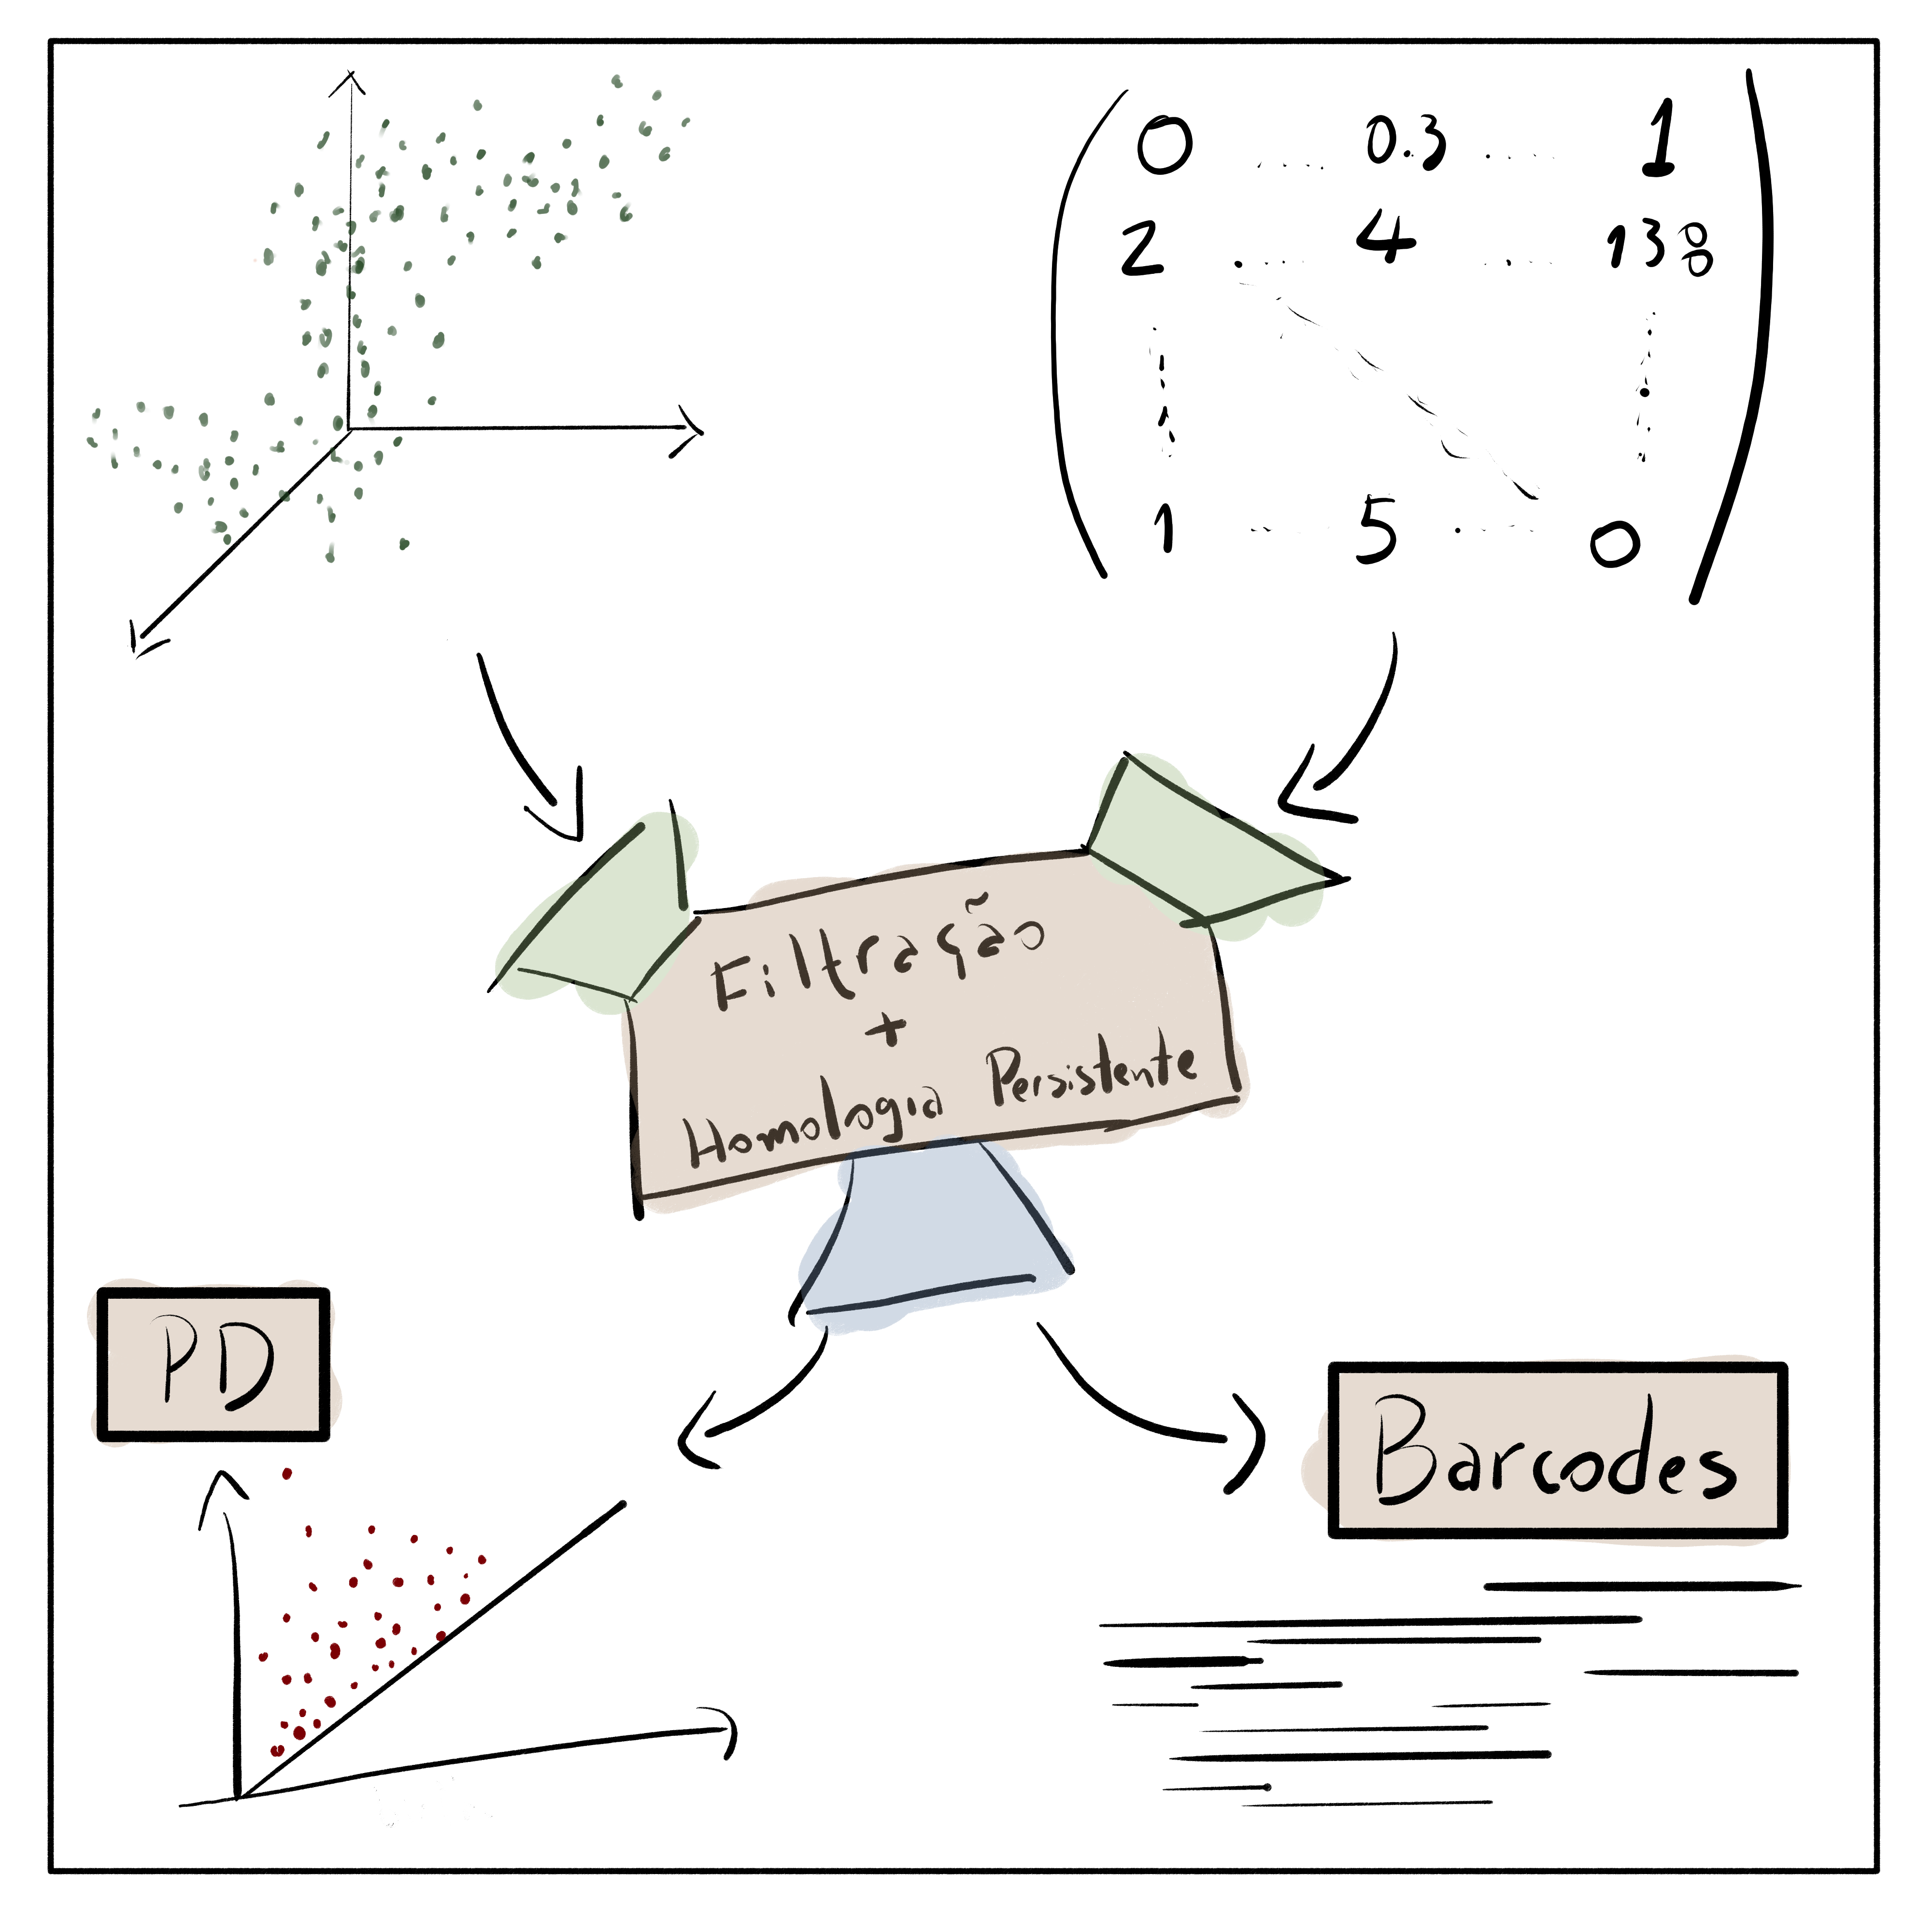
\includegraphics[width=0.7\textwidth]{images/pipeline_hp.png}
  \caption{Representação do pipeline para a utilização da homologia persistente
          com um conjunto de dados.}
  \label{fig:pipeline_hp}
\end{figure}


\section{Filtrações e espaços vetoriais}
A filtração de um conjunto de dados é o primeiro passo na nossa sequência apresentada
na~\autoref{fig:pipeline_hp}.
Dado um conjunto de dados precisamos construir um objeto combinatorial de forma
que possa ser analisado do ponto de vista da topologia assim como computacionalmente.
A filtração é este objeto que captura as mudanças do conjunto dada uma escala.

Algumas definições se fazem necessárias para entendermos o que é a filtração
e qual o seu papel na análise topológica de dados. Começamos definindo um simplexo,
primeiro objeto combinatorial que é a base da filtração.

\begin{defi}
  Sejam $v_0, v_1, \dots, v_k \in \mathbb{R}^n$ linearmente afins, ou seja $\{v_1 - v_0, \dots, v_k - v_0\}$
  é um conjunto linearmente independente. O k-simplexo definido pelos pontos acima
  definidos, chamados de vértices também, é o conjunto

  \begin{equation*}
    \Set{\sum_{i=0}^k \lambda_i v_i \ | \ \sum_{i=0}^k \lambda_i = 1 \text{ e }
          \lambda_i \ge 0, \ \forall i}.
  \end{equation*}
\end{defi}

Note que para $k = 0$, temos um único vértice. Para $k=1$, temos uma reta, já
para $k=2$ temos um triângulo preenchido. E no caso $k=3$, um tetraedro. Os
simplexos podem ser vistos na~\autoref{fig:ksimpl}. Além disso, dizemos que a dimensão
do $k$-simplexo é $k$. A envoltoria convexa de qualquer subconjunto dos vértices
de um simplexo $S$ é chamado de face de $S$.

\begin{figure}
  \centering
  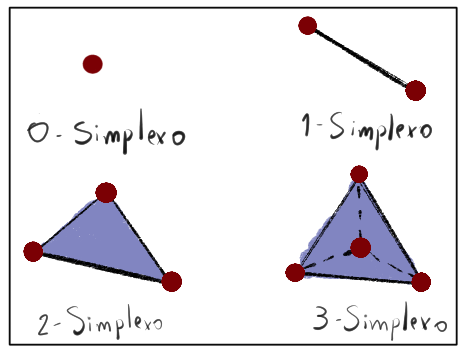
\includegraphics[width=0.7\textwidth]{images/ksimpl.png}
  \caption{Exemplos de $k$-simplexos para $k\in \Set{0,1,2,3}$.}
  \label{fig:ksimpl}
\end{figure}

Tendo definido os $k$-simplexos, podemos definir o complexo simplicial.
\begin{defi}
    Um complexo simplicial $K$ é uma coleção de simplexos satisfazendo as seguintes
    relações:
    \begin{itemize}
      \item Dado $\sigma \in K$, temos que para toda face $\tau \subset \sigma$
            vale $\tau \in K$.
      \item A interseção de dois simplexos é face de ambos os simplexos, em outras palavras,
      $\sigma, \tau \in K$ implica que $\sigma \cap \tau \subset \sigma$ e
      $\sigma \cap \tau \subset \tau$.
    \end{itemize}
\end{defi}
A segunda condição é necessária para evitar casos patológicos como mostrado na
\autoref{fig:simp_path}

\begin{figure}
  \centering
  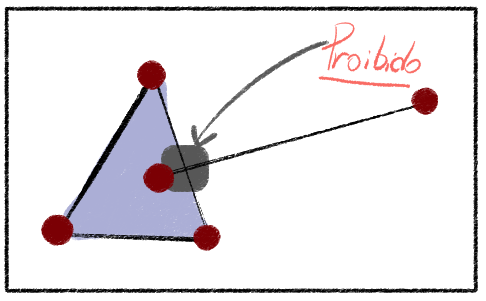
\includegraphics[width=0.7\textwidth]{images/simp_path.png}
  \caption{Exemplo em que a interseção de dois simplexos não é um simplexo.}
  \label{fig:simp_path}
\end{figure}
Dizemos que a dimensão do complexo simplicial $K$ é a maior dimensão dentre os
simplexos em $K$. Podemos definir agora a filtração de um complexo simplicial.

\begin{defi}
  Seja $K$ um complexo simplicial. Definimos uma filtração de $K$ sendo uma
  sequência de subconjuntos $K_i \subset K$, com $i \in \{ 1, \dots, n \}$,
  de tal forma que $K_i$ é um complexo simplicial para todo $i$ e vale que
  \begin{equation*}
    K_1 \subset \dots \subset K_{n-1} \subset K_n = K.
  \end{equation*}
\end{defi}
Na~\autoref{fig:filtracao_exemplo} temos um exemplo de filtração para um complexo
simplicial.

\begin{figure}[hbt]
  \centering
  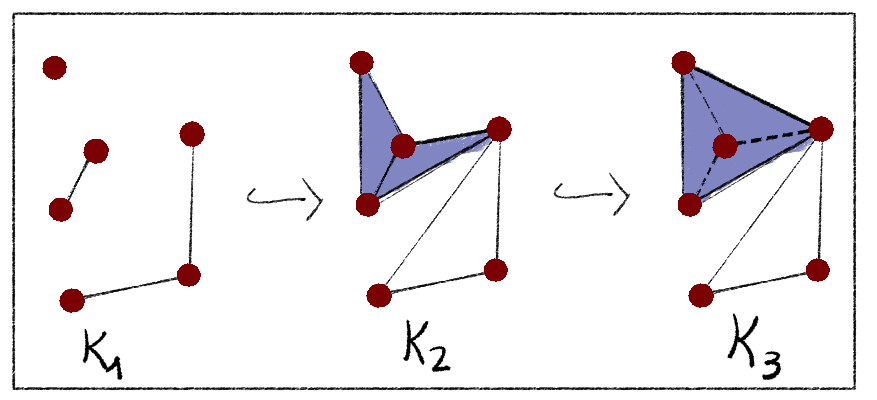
\includegraphics[width=0.7\textwidth]{images/filtracao_exemplo.png}
  \caption{Exemplo de filtração para um complexo simplicial $K$.}
  \label{fig:filtracao_exemplo}
\end{figure}

A pergunta que temos agora é como construir uma filtração dado um conjunto
de dados? E felizmente temos várias respostas para isso.


\section{A matriz de bordo $\partial$}

\section{Redução da matriz}


\chapter{Módulos de Persistência}
\label{chapter:mph}
A homologia persistente teve seu ínicio em uma intersecção entre as ciências da computação 
e a matemática. Os primeiros artigos mostravam algoritmos sobre espaços topológicos simples,
como esferas \cite{Edelsbrunner2000}. No entanto, a teoria foi se desenvolvendo 
ao longo dos anos ao ponto em que as linguagens utilizadas para tratar da homologia persistente 
é a teoria de categorias conjuntamente com a teoria de representações \cite{Chazal2016}.

Neste capítulo tratamos do desenvolvimento da homologia persistente sob a luz dessas linguagens. 
Na primeira seção definimos o que são os módulos de persistência e suas relações com os diagramas de 
persistência. Na segunda seção descrevemos a medida retangular, usada para abstrair o conceito 
de diagrama de persistência e poder estudar o quão \textit{tame} ele o é. Apresentamos na terceira seção
alguns exemplos do comportamento dos módulos de persistência e exemplos. A quarta seção é fundamental,
pois mostramos como comparar dois módulos de persistência, através do \textit{interleaving}. E finalmente,
apresentamos o teoria de isometria e mostramos uma das implicações com a teoria desenvolvido neste capítulo. 

\section{Módulos de persistência e decomposições}
Nesta seção iremos definir os módulos de persistência, apresentar teoremas de decomposição dos módulos 
e introduzir a notação de quiver, que será utilizada para as próximas seções e demonstrações de 
outros resultados. 

Fixaremos aqui o corpo $\mathbf{k}$ para todos os espaços vetoriais apresentados neste texto. 

\begin{defi}
    Um módulo de persistência $\mathfrak{V}$ sobre os números reais $\mathbb{R}$ é uma família indexada 
    sobre $\mathbb{R}$ de espaços vetoriais 
    \begin{equation*}
        (V_t \mid t \in \mathbb{R}), 
    \end{equation*} 
    e uma família de aplicações lineares duplamente indexadas
    \begin{equation*}
        (v_t^s \colon V_s \to V_t \mid s \leq t) 
    \end{equation*}
    que satisfazem a seguinte relação de composição
    \begin{equation*}
        v_t^s \circ v_s^r = v_t^r,
    \end{equation*} 
    em que a função $v^r_r$ é considerada a função identidade. 
\end{defi}

O módulo de persistência pode ser visto como um funtor entre a categoria dos números reais com o morfismo
$s \to t$, em que $s \leq t$ e a categoria de espaços vetoriais. 

Vamos dar um exemplo de módulo de persistência que se encontra no contexto de análise topológica de dados. 
Seja $X$ um espaço vetorial e $f \colon X \to \mathbb{R}$ uma função, não necessariamente contínua e 
considere os conjuntos de nível
\begin{equation*}
    X^t = (X,f)^t = \Set{x \in X \mid f(x) \leq t}.
\end{equation*}

Temos uma sequência de conjuntos encaixados, $X^t$ com $t \in \mathbb{R}$, ou seja, existe uma função 
inclusão $\iota_t^s \colon X^s \hookrightarrow X^t$ que satisfaz trivialmente a lei de composição e 
existe uma função identidade. Chamamos esta sequência de conjuntos e funções de filtração de subníveis
de $(X,f)$, denotada por $\mathfrak{X}_{sub}$ ou $\mathfrak{X}^f_{sub}$.

Dada a sequência acima, podemos transforma-la em um módulo de persistência utilizando qualquer funtor
da categoria de espaços topológicos para a categoria de espaços vetoriais. Neste caso utilizamos 
o funtor de homologia $H = H_k(-, \mathbf{k})$ de dimensão $k$ com coeficientes em $\mathbf{k}$. Assim,
podemos definir o seguinte módulo de persistência $\mathfrak{V}$

\begin{equation*}
    V_t = H(X^t) \qquad v^s_t = H(\iota_t^s) \colon V_s \to V_t.
\end{equation*}
Podemos também escrever $\mathfrak{V} = H(\mathfrak{X}_{sub})$. 

Um exemplo na análise topológica de dados é quando $X$ é um complexo simmplicial finito e $X^t$ é um 
subcomplexo. Devido as propriedades dos complexos, existem finitos valores críticos onde há mudanças 
em $X$. Suponha que os valores sejam $a_1 < \dots < a_n$. Entao toda a informação do módulo de 
persistência é dada pela seguinte sequência de espaços vetoriais de dimensão finita

\begin{equation*}
    H(X^{a_1}) \to \dots \to H(X^{a_n}).
\end{equation*}

Neste caso, $H(\mathfrak{X}_{sub})$ admite uma descrição compacta, existe um algoritmo eficiente para 
o seu calculo e por último, a descrição é contínua com relação a $f$, ou seja, é estável sob uma 
métrica. 

A descrição mencionada acima é o diagrama de persistência ou barcode. A estrutura é dada por uma 
lista de intervalos da forma $[b,d) = [a_i, a_j)$ ou $[a_i, +\infty)$. Cada intervalo representa
um ciclo, uma propriedade, que nasce em $b$ e morre em $d$. 

Iremos mostrar aqui que é possível associar um diagram de persistência para módulos de 
persistência $\mathfrak{V}$ \textit{q-tame}. Um módulo de persistência é \textit{q-tame} 
se 
\begin{equation*}
    r_t^s = \text{rank}(v_t^s) < \infty \text{ para } s < t.
\end{equation*}
Intuitivamente falando, um módulo é \textit{q-tame} se para todo quadrante que pegamos com a origem
na diagonal, existem finitos pontos do diagram de persistência neste quadrante como pode ser visto
na \autoref{fig:quad_finito}.

\begin{figure}
    \centering
    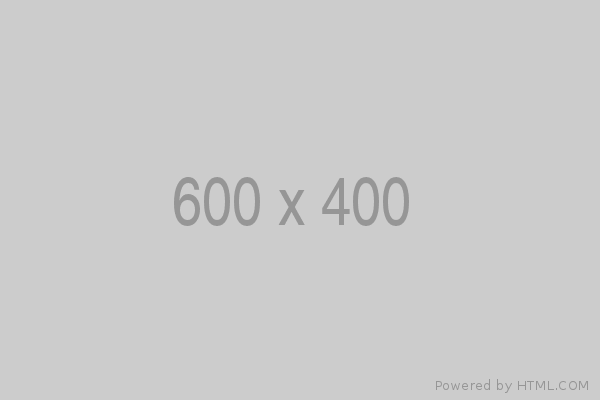
\includegraphics[width=0.5\textwidth]{images/placeholder.png}
    \caption{Exemplo de um diagram de persistência de um módulo de 
            persistência \textit{q-tame} com um quadrante em destaque.}
    \label{fig:quad_finito}
\end{figure}

\subsection{Indíces e posets} 
No início desta seção definimos o módulo de persistência com o conjunto de indíces sendo os reais. No 
entanto, é possível definir utilizando quaisquer conjuntos parcialmente ordenados da mesma forma que 
com os reais. Seja $\mathbf{T}$ um poset, a coleção de espaços vetoriais e aplicações lineares que 
satisfazem as leis de composição e identidade é chamada de $\mathbf{T}$-módulo de persistência, ou 
módulo de persistência sobre $\mathbf{T}$. 

Além disso, podemos restringir o poset $\mathbf{T}$ para um subconjunto $\mathbf{S} \subset \mathbf{T}$
de forma a obter o $\mathbf{S}$-módulo de persistência, que são os espaços vetoriais e aplicações lineares
cujos indíces são elementos de $\mathbf{S}$. Esta é a restrição de $\mathfrak{V}$ em $\mathbf{S}$ e pode
ser denotada por $\mathfrak{V}_S$ ou $\left.\mathfrak{V}\right|_S$. 

\subsection{Categoria de módulos}
Com a definição de módulos de persistência sobre um poset $\mathbf{T}$ qualquer, podemos definir
homomorfismos entre módulos. Sejam $\mathfrak{U}, \mathfrak{V}$ $\mathbf{T}$-módulos de persistência.
Um homomorfismo $\Phi$ entre $\mathfrak{U}$ e $\mathfrak{V}$ é uma família de aplicações lineares 
$(\phi_t \colon U_t \to V_t \mid t \in \mathbf{T})$ tal que o seguinte diagrama comuta para todo
$s \leq t$. 

\begin{equation*}
    \begin{tikzcd}
        U_s \arrow{d}[swap]{\phi_s} \arrow{r}{u_t^s} & U_t \arrow{d}{\phi_t} \\
        V_s \arrow{r}{v^s_t}                     & V_t                    
    \end{tikzcd} 
\end{equation*}

A composição de dois homomorfismo $\Phi, \Psi$ é dada por cada indíce $t \in \mathbf{T}$, ou seja,
$\Phi \circ \Psi$ é a coleção de aplicações lineares $(\phi_t \circ \psi_t \colon U_t \to W_t \mid t \in \mathbf{T})$,
onde $\Phi$ é homomorfismo entre $\mathfrak{U}$ e $\mathfrak{V}$ e $\Psi$ entre $\mathfrak{V}$ e $\mathfrak{W}$. 
A identidade é definida de forma trivial. Portanto, temos a categoria dos módulos. Definamos os seguintes conjuntos
\begin{align*}
    \text{Hom}(\mathfrak{U}, \mathfrak{V}) &= \Set{\text{homomorfismos } \mathfrak{U} \to \mathfrak{V}}, \\
    \text{End}(\mathfrak{V}) &= \Set{\text{homomorfismos } \mathfrak{V} \to \mathfrak{V}}.
\end{align*}

\subsection{Módulos Intervalares}
A relação entre os diagramas de persistência e módulos de persistência são fundamentadas pelos módulos intervalares. 
Eles são a base da teoria de homologia persistente. 

Um intervalo em um conjunto totalmente ordenado $\mathbf{T}$ é um subconjunto $J \subset \mathbf{T}$ tal que se 
$r \in J$ e $t \in J$ tal que $r < s < t$, então $s \in J$. Portanto, para qualquer intervalo $J \subset \mathbf{T}$,
o módulo intervalar $\mathfrak{I} = \mathbf{k}^J$ é definido como o $\mathbf{T}$-módulo de persistência com a 
seguinte família de espaços vetoriais
\begin{equation*}
    I_t = \left\{
    \begin{split}
        & \mathbf{k} \text{ se } t \in J \\
        & 0 \text{ caso contrário,}
    \end{split}
    \right.
\end{equation*} 
e as aplicações lineares
\begin{equation*}
    i_t^s = \left\{
    \begin{split}
        & id \text{ se } s,t \in J \\
        & 0 \text{ caso contrário.}
    \end{split}
    \right.
\end{equation*}
Como mencionado anteriormente, os intervalos seriam as propriedades representadas no diagrama de persistência, 
ou seja, o módulo intervalar $\mathbf{k}^J$ representa uma propriedade que persiste por todo intervalo $J$.

Devida a sua importância, módulos intervalares com índices em subconjuntos de $\mathbb{R}$ possuem uma notação 
especial. Para distinguir os vários casos de intervalos, usamos uma supernotação: $+$ e $-$, a decoração dos pontos.
Para intervalos finitos adota-se o seguinte dicionário

\begin{align*}
    (p^-, q^-) &= [p,q) \\ 
    (p^-, q^+) &= [p,q] \\
    (p^+, q^-) &= (p,q) \\
    (p^+, q^+) &= (p,q]
\end{align*}
O dicionário acima vale para $p < q$. No caso em que $p=q$, representamos o intervalo por $(p^-, p^+) = [p,p]$. 
Para intervalos infinitos, usamos o símbolo $-\infty^+$ e $+\infty^-$ com definição similar à acima e com a adição
do seguinte intervalo
\begin{equation*}
    (-\infty^+, +\infty^-) = (-\infty, +\infty).
\end{equation*}
Quando queremos referenciar um ponto decorados mas não sabemos sua decoração, denotamos por $p^*$, podendo ser 
$p^-$ ou $p^+$. 

Podemos extender os reais para os reais decorados, um conjunto totalmente ordenado com as seguintes relações
\begin{equation*}
    p^- < p < p^+ < q^- < q < q^+,
\end{equation*}
para todo $p < q$. Definimos o semiplano diagonal superior em $\mathbb{R}^2$ como 
\begin{equation*}
    \mathcal{H} = \Set{(p,q) | p \leq q}
\end{equation*}
O semiplano diagonal superior $\bar{\mathcal{H}}$ é a união de $\mathcal{H}$ com os pontos no infinito. 

Portanto, um módulo intervalar pode ser representado de diversas formas, visualizados também na \autoref{fig:mod_int}
\begin{itemize}
    \item Como um intervalo na reta real;
    \item como uma função $\mathcal{H} \to \Set{0,1}$ definida por $(s,t) \mapsto \text{rank}(i^s_t)$; 
    \item como um ponto $(p,q) \in \mathcal{H}$ e um traço representando a respectiva decoração.
\end{itemize}
 
\begin{figure}[htpb!] 
    \centering
    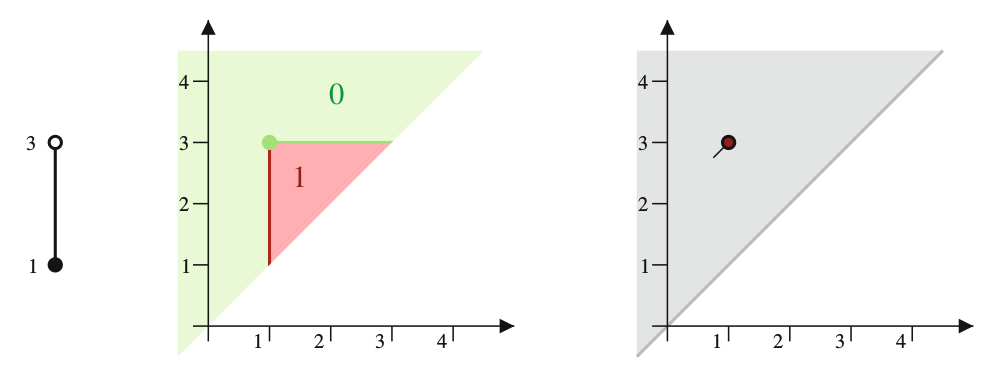
\includegraphics[width=0.7\textwidth]{images/ex_interval_module.png}
    \caption{Representação por intervalo (esquerda), pela função rank (meio) e pelo ponto decorado (direita) do 
            módulo intervalar $\mathbf{k}[1,3) = \mathbf{k}(1^-, 3^-)$.}  
    \label{fig:mod_int}
\end{figure}
Os traços representando a decoração são dados por
\begin{center}
    $(p^-,q^-): $ \rotatebox[origin=c]{225}{$\multimap$}

    $(p^-,q^+): $ \rotatebox[origin=c]{135}{$\multimap$}

    $(p^+,q^-): $ \rotatebox[origin=c]{315}{$\multimap$}

    $(p^+,q^+): $ \rotatebox[origin=c]{45}{$\multimap$}
\end{center}

\subsection{Decomposição em módulos intervalares} 

\begin{defi}
    A \textbf{soma direta} $\mathfrak{W} = \mathfrak{U} \oplus \mathfrak{V}$ de dois módulos
    de persistência $\mathfrak{U}$ e $\mathfrak{V}$ é definida por
    \begin{equation*}
        W_t = U_t \oplus V_t, \quad w^s_t = u_t^s \oplus v^s_t
    \end{equation*}
\end{defi}
Esta definição generaliza-se para somar arbitrárias, tanto finitas como infinitas. Vamos agora definir
a indecomponibilidade de um módulo de persistência.

\begin{defi}
    Um módulo de persistência $\mathfrak{W}$ é indecomponível se dada uma decomposição $\mathfrak{U}
    \oplus \mathfrak{V}$, então $\mathfrak{U} = 0$ ou $\mathfrak{W}$ e $\mathfrak{V} = 0$ ou $
        \mathfrak{W}$.
\end{defi}

Podemos estudar os módulos de persistência através de sua decomposição por módulos intervalares. Dado
uma sequência de intervalos $(J_l \mid l \in L)$,
\begin{equation*}
    \mathfrak{V} \cong \bigoplus_{l \in L} \mathbf{k}^{J_l}.
\end{equation*}
Neste caso, podemos pensar que cada intervalo $J_l$ representa uma propriedade. Esta decomposição acaba
sendo muito importante por este motivo. Mas a questão que fica é: quais módulos são decomponíveis em 
intervalos? E porque decompõe-se em módulos intervalares? 

A resposta para a primeira pergunta é o Teorema \ref{teo:crawley}. Já para a segunda questão,
os módulos intervalares são indecomponíveis, como mostramos na Proposição \ref{prop:mod_int}.

\begin{propo}
    Seja $\mathfrak{I} = \mathbf{k}^J_T$ um módulo intervalar sobre $\mathbf{T} \subset \mathbb{R}$. 
    Então $\text{End}(\mathfrak{I}) = \mathbf{k}$. 
\end{propo}
\begin{proof}
    Vamos definir uma função $\Phi$ entre $\text{End}(\mathfrak{I})$ e $\mathbf{k}$ que será um isomorfismo
    de aneis.
    Seja $\Phi \colon \mathbf{k} \to \text{End}(\mathfrak{I})$ definida por 
    \begin{equation*}
        \alpha \mapsto \varphi^{\alpha}
    \end{equation*}
    onde $\varphi^\alpha$ é um endomorfismo de $\mathfrak{I}$ tal que $\varphi_t^{\alpha} \colon I_t 
    \to I_t$ e $\varphi^{\alpha}_t (x) = \alpha x$. É fácil ver que a aplicação é um homomorfismo de anéis.
    Vamos definir a inversa de $\Phi$. Para isso, note primeiro que qualquer endomorfismo de $\mathfrak{I}$
    age como multiplicação por escalar em qualquer $I_t$ não nulo. Precisamos mostrar que dados $s,t$, temos 
    que o escalar definido é o mesmo para ambos os casos:
    \begin{align*}
        \Psi^{-1} \colon & \mathfrak{I} \to \mathbf{k} \\
                         & \varphi \mapsto \alpha,
    \end{align*}
    Vamos mostrar que a aplicação está bem definida.
    
    Primeiro, pela observação acima, dados $s,t$ tais que $I_s, I_t \neq 0$, temos que vale o seguinte
    para $\varphi \in \mathfrak{I}$.
    \begin{align*}
        \varphi_s \colon & \mathbf{k} \to \mathbf{k} \\
                         &     x \mapsto \alpha x 
    \end{align*}
    e 
    \begin{align*}
        \varphi_t \colon & \mathbf{k} \to \mathbf{k} \\
                         &     x \mapsto \beta x 
    \end{align*}
    Precisamos mostrar que $\alpha = \beta$, demonstrando a proposição. Mas isso segue pelo 
    diagrama comutativo dos homomorfismos entre módulos de persistência, como podemos ver na 
    Eq. \eqref{eq:diag_prop_end}, assumindo que $s \leq t$. 
    \begin{equation}
        \label{eq:diag_prop_end}
        \begin{tikzcd}
            I_s \arrow{d}[swap]{\varphi_s} \arrow{r}{id} & I_t \arrow{d}{\varphi_t} \\
            I_s \arrow{r}{id}                     & I_t                    
        \end{tikzcd} 
    \end{equation}
    No caso acima temos a identidade entre $I_s$ e $I_t$, já que ambos são $\mathbf{k}$. Logo,
    segue que $\alpha=\beta$, provando a Proposição.
\end{proof}

\begin{propo}\label{prop:mod_int}
    Módulos intervalares são indecomponíveis. 
\end{propo}
\begin{proof}
    Suponha que exista uma decomposição $\mathfrak{I} = \mathfrak{U} \oplus \mathfrak{V}$. Considere agora
    as projeções sob $\mathfrak{U}$ e $\mathfrak{V}$. Ambas são homomorfismos idempotentes. Mas como 
    $\text{End}(\mathfrak{I})$ é isomorfo a $\mathbf{k}$ e os únicos idempotentes de $\mathbf{k}$ são 
    $0$ e $1$, segue que $\mathfrak{I}$ é indecomponível. 
\end{proof}

\begin{teo}{(Krull-Remak-Schmidt-Azumaya)}\label{teo:krull}
    Suponha que um módulo de persistência $\mathbf{T} \subset \mathbb{R}$ pode ser escrito como soma 
    direta de módulos intervalores de duas formas diferentes
    \begin{equation*}
        \mathfrak{V} \cong \bigoplus_{l \in L} \mathbf{k}^{J_l} \cong \bigoplus_{m \in M} \mathbf{k}^{K_m},
    \end{equation*}
    então existe uma bijeção $\sigma \colon L \to M$ tal que $J_l = K_{\sigma(l)}$ para todo $l \in L$. 
\end{teo}
\begin{proof}
    A demonstração segue do Teorema $1$~\cite{Azumaya1950} com a observação de que se $\mathbf{k}^J \cong 
    \mathbf{k}^L$, então $J=K$. Só é necessário verificar uma condição de localidade para aplicarmos o teorema:
    se $\psi, \phi \in \text{End}(\mathfrak{I})$ são não isomorfismos, então $\psi + \phi$ não é isomorfismo. 
    Mas pela proposição anterior, isso segue do fato que a unica aplicação que não é isomorfismo em 
    $\text{End}(\mathfrak{I})$ é a aplicação nula.
\end{proof}

\begin{teo}{(Gabriel, Auslander, Ringel-Tachikawa, Webb, Crawley-Boevey)}\label{teo:crawley}
    Seja $\mathfrak{V}$ um módulo de persistência sobre $\mathbf{T} \subset \mathbb{R}$. Então $\mathfrak{V}$
    pode ser decomposto como um soma direta de módulos intervalares sob as seguintes condições:
    \begin{itemize} 
        \item $\mathbf{T}$ é um conjunto finito;
        \item cada $V_t$ é um espaço vetorial de dimensão finita. 
    \end{itemize}
    Por outro lado, existe um módulo de persistência sob $\mathbb{Z}$ que não admite uma decomposição intervalar. 
\end{teo}  
\begin{proof}
    Detalhes podem ser vistos em \cite{Chazal2016}, página 22, \textbf{Teorema} 2.8.
\end{proof}

Se um módulo de persistência indexado sobre $\mathbb{R}$ pode ser decomposto
\begin{equation*}
    \mathfrak{V} \cong \bigoplus_{l \in L} \mathbf(p_l^*, q_l^*),
\end{equation*}
então o diagrama de persistência decorado é definido pelo multiconjunto
\begin{equation*}
    \text{Dgm} (\mathfrak{V}) = \text{Int}(\mathfrak{V}) = \Set{(p_l^*, q_l^*) | l \in L}
\end{equation*}
e o diagram de persistência não decorado é o multiconjunto
\begin{equation*}
    \text{dgm} (\mathfrak{V}) = \text{int}(\mathfrak{V}) = \Set{(p_l, q_l) | l \in L} - \Delta,
\end{equation*}
onde $\Delta$ é a diagonal no plano.

Note que ambos os diagramas definidos não dependem da escolha da decomposição, devido ao Teorema \ref{teo:krull}. 
Além disso, o diagrama dgm é o diagrama de pontos não decorados e sem a diagonal, sendo encontrado com 
frequência em exemplos práticos de análise de dados. Para a definição da distância bottleneck acaba sendo 
mais importante. 

\subsection{Cálculos com quivers}

Vamos agora definir uma notação para trabalhar com módulos de persistência sobre conjuntos de índices 
finitos. 
Um módulo de persistência $\mathfrak{V}$ sobre um conjunto finito de índices
\begin{equation*}
    \mathbf{T} : \qquad a_1 < \dots < a_n 
\end{equation*} 
da reta real pode ser visto como um diagrama de $n$ espaços vetoriais e $n-1$ aplicações lineares, como
mostrado abaixo
\begin{equation*}
    \mathfrak{V} : \quad V_{a_1} \longrightarrow \dots \longrightarrow V_{a_n}.
\end{equation*}
O diagrama acima é a representação do seguinte \textbf{quiver}:
\begin{equation*}
    \bullet \longrightarrow \bullet \longrightarrow \dots \longrightarrow \bullet
\end{equation*}

Vimos que podemos decompor alguns módulos de persistência em módulos intervalares. Para estes podemos representa-los 
com quivers da seguinte forma. 
\begin{ex}
    Seja $a < b < c$. Existem $6$ módulos intervalares diferentes sobre este intervalo.
\begin{equation*} 
    \begin{matrix}
        \mathbf{k}[a,a] = \qon{a} \qem \qoff{b} \qem \qoff{c} & \mathbf{k}[a,b] = \qon{a} \qem \qon{b} \qem \qoff{c}& 
                            \mathbf{k}[a,c] = \qon{a} \qem \qoff{b} \qem \qon{c}\\
        \mathbf{k}[b,b] = \qoff{a} \qem \qon{b} \qem \qoff{c}& \mathbf{k}[b,c] = \qoff{a} \qem \qon{b} \qem \qon{c}& \\
        \mathbf{k}[c,c] = \qoff{a} \qem \qoff{b} \qem \qon{c}& & & 
    \end{matrix}
\end{equation*}
\end{ex}

Os círculos $\bullet$ representam uma cópia do espaço vetorial $\mathbf{k}$ unidimensional. O círculo $\circ$ representa o 
espaço vetorial nulo. A aplicação linear entre dois $\bullet$ é a identidade e qualquer aplicação contendo $\circ$ é a
nula.

Esta notação pode ser usada para representar a multiplicidade dos módulos intervalares da decomposição
de um módulo de persistência sobre um conjunto de índices finito, essa quando existe. Seja $\mathfrak{V}$
um módulo de persistência sobre o conjunto $\mathbf{T} = \Set{a_1, \dots, a_n}$. Definimos a multiplicidade
de $[a_i, a_j] \subseteq \mathbf{T}$ em $\mathfrak{V}_{\mathbf{T}}$ como o número de cópias do módulo
$\mathbf{k}[a_i,a_j]$ na decomposição de $\mathfrak{V}_{\mathbf{T}}$. 

\begin{ex}
    Seja $\mathfrak{V}$ módulo de persistência sobre $\mathbf{T} = \Set{a,b,c}$. Escrevemos
    \begin{equation*}
        \innerproduct{[b,c] \mid \mathfrak{V}_{\mathbf{T}}} \text{ ou } \innerproduct{\qoff{a} \qem \qon{b} 
        \qem \qon{c} \mid \mathfrak{V}}
    \end{equation*}
    para representar a multiplicidade de $\qoff{a} \qem \qon{b} \qem \qon{c}$ no seguinte módulo de $3$ termos
    \begin{equation*}
        \mathfrak{V} : \quad V_{a_1} \longrightarrow \dots \longrightarrow V_{a_n}.
    \end{equation*}
\end{ex}

\begin{ex}
    Considere o módulo com dois espaços vetoriais e uma única aplicação linear $\mathfrak{V} : \quad 
    V_a \xrightarrow{\mu} V_b$. Então os invariantes de $\mu$ são
    \begin{align*}
        \text{rank}(\mu)       & = \innerproduct{\qon{a} \qem \qon{b} \mid \mathfrak{V}}, \\
        \text{nulidade}(\mu)   & = \innerproduct{\qon{a} \qem \qoff{b} \mid \mathfrak{V}}, \\
        \text{conulidade}(\mu) & = \innerproduct{\qoff{a} \qem \qon{b} \mid \mathfrak{V}}.
    \end{align*}
    Basta notar que para $V_a, V_b$ espaços de dimensão finita, existe uma decomposição das suas bases 
    \begin{equation*}
        e_1, \dots, e_r, f_1, \dots, f_n \text{   e   } g_1, \dots, g_r, h_1, \dots, h_m
    \end{equation*}
    tais que $\mu(e_i) = g_i$, $\mu(f_j) = 0$ para todo $i,j$. Assim, os espaços vetoriais unidimensionais
    gerados pelos elementos das bases geram uma decomposição do módulo $\mathfrak{V}$ nos seguintes intervalos
    \[\begin{array}{ccccc}
        (&\text{span}(e_i) & \rightarrow &\text{span}(g_i)&) \\
        (&\text{span}(f_j) & \rightarrow &0               &) \\
        (& 0               & \rightarrow &\text{span}(h_k)&)
    \end{array}\]
    que são isomorfos respectivamente à $\qon{a} \qem \qon{b}$, $\qon{a} \qem \qoff{b}$ e 
    $\qoff{a} \qem \qon{b}$. 
\end{ex}

\begin{propo}\label{teo:direct_sum}
    Suponha que podemos decompor um módulo de persistência $\mathfrak{V}$ como uma soma direta
    \begin{equation*}
        \mathfrak{V} = \bigoplus_{l\in L} \mathfrak{V}^l,
    \end{equation*}
    então 
    \begin{equation*}
        \langle [a_i, a_j] \mid \mathfrak{V}_{\mathbf{T}} \rangle = \sum_{l\in L} \langle [a_i, a_j] 
        \mid \mathfrak{V}_{\mathbf{T}}^l \rangle
    \end{equation*}
    para qualquer conjunto de índices $\mathbf{T} = \Set{a_1, \dots, a_n}$ e intervalos $[a_i, a_j] \subseteq \mathbf{T}$.
\end{propo}
\begin{proof}
    Segue do fato que a decomposição intervalar de $\mathfrak{V}_{\mathbf{T}}$ é a soma direta das decomposições intervalares 
    de cada $\mathfrak{V}^l_{\mathbf{T}}$ para todo $l \in L$. 
\end{proof}

\begin{propo}{(Princípio da restrição)}\label{teo:restr_princ}
    Sejam $\mathbf{S}, \mathbf{T}$ conjuntos de índices com $\mathbf{S} \subset \mathbf{T}$. Então
    \begin{equation*}
        \langle I \mid \mathfrak{V}_{\mathbf{S}} \rangle = 
        \sum_{J} \langle J \mid \mathfrak{V}_{J} \rangle,
    \end{equation*}
    onde a soma é sobre todos os intervalos $J \subseteq \mathbf{T}$ que se restringe a 
    $I$ sobre $\mathbf{S}$. 
\end{propo}
\begin{proof}   
    Tome uma decomposição intervalar arbitrária de $\mathfrak{V}_{\mathbf{T}}$. Então uma decomposição
    intervalar é induzida em $\mathfrak{V}_{\mathbf{S}}$. Note agora que para $I \subseteq \mathbf{S}$,
    temos diversos intervalos $J \subseteq \mathbf{T}$ tais que $J \cap \mathbf{S} = I$. Devido a 
    linearidade da soma direta, temos que os intervalos de $\mathfrak{V}_{\mathbf{S}}$ do tipo $I$ 
    são os intervalos de $\mathfrak{V}_{\mathbf{T}}$ do tipo $J$ acima. 
\end{proof}
\begin{ex}
    Seja $a < p < b < q < c$. Então temos os seguintes exemplos para os conjuntos de índices:
    \begin{itemize}
        \item $\mathbf{T}_1 = \Set{a,b,q,c}$, $S_1=\Set{a,b,c}$, $I_1=[b,c]$.
        \begin{equation*}
            \innerproduct{\qoff{a} \qem \qno \qem \qon{b} \qem \qno \qem \qon{c}} =
            \innerproduct{\qoff{a} \qem \qno \qem \qon{b} \qem \qon{q} \qem \qon{c}} 
        \end{equation*}
        \item $\mathbf{T}_2 = \Set{a,p,b,c}$, $S_2=\Set{a,b,c}$, $I_2=[b,c]$.
        \begin{equation*}
            \innerproduct{\qoff{a} \qem \qno \qem \qon{b} \qem \qno \qem \qon{c}} =
            \innerproduct{\qoff{a} \qem \qoff{p} \qem \qon{b} \qem \qno \qem \qon{c}}
            + \innerproduct{\qoff{a} \qem \qon{p} \qem \qon{b} \qem \qno \qem \qon{c}} 
        \end{equation*}
        \item $\mathbf{T}_3 = \Set{a,b,q,c}$, $S_2=\Set{a,b,c}$, $I_2=[c,c]$.
        \begin{equation*}
            \innerproduct{\qoff{a} \qem \qno \qem \qoff{b} \qem \qno \qem \qon{c}} =
            \innerproduct{\qoff{a} \qem \qno \qem \qoff{b} \qem \qoff{q} \qem \qon{c}}
            + \innerproduct{\qoff{a} \qem \qno \qem \qoff{b} \qem \qon{q} \qem \qon{c}} 
        \end{equation*}
         
    \end{itemize}
\end{ex}

\section{Medidas retangulares}
Na seção anterior discutimos módulos de persistência decomponíveis e seus diagramas de persistência,
Dgm e dgm. No entanto, nem sempre os módulos são decomponíveis, não sendo possível definir os 
diagramas de persistência. Para definir-los, podemos nos guiar pela seguinte ideia: se soubermos 
contar o número de pontos do Dgm pertence em cada retângulo do semiplano, então conhecemos Dgm.

Iremos nos inspirar na teoria da medida para construir uma função que nos dá um valor inteiro ou 
infinito e que podemos associar um diagrama de persistência com ela. A ideia é que para módulos 
bem comportados podemos avaliar esta função em retângulos e extrair um conjunto discreto de pontos,
que juntamente com sua multiplicidade gerará o diagrama de persistência. No caso que o módulo de 
persistência for decomponível, as definições são iguais. Caso contrário seguimos com a teoria 
normalmente. 

No resto deste capítulo iremos tratar apenas de medidas finitas no semiplano diagonal sem considerar
os pontos no infinito. Os argumentos usados podem ser facilmente estendidos para o caso de medidas
infinitas através de um processo de limite e para o semiplano diagonal com os pontos no infinito 
podemos usar o truque de colocar tudo dentro de um retângulo com a função $\arctan$.
 
\subsection{A medida de persistência}

\begin{defi} 
    Seja $\mathfrak{V}$ um módulo de persistência. Então a medida de persistência de $\mathfrak{V}$ é a função
    \begin{equation*}
        \mu_{\mathfrak{V}}(R) = \innerproduct{\qoff{a} \qem \qon{b} \qem \qon{c} \qem \qoff{d} \mid \mathfrak{V}}
    \end{equation*}
    definida no retângulo $R = [a,b]\times[c,d]$ no plano com $a < b \leq c < d$. 
\end{defi}

Veremos como a medida tem uma relação com módulos decomponíveis. Abaixo um resultado para módulos intervalares.

\begin{propo}\label{teo:int_meas}
    Seja $\mathfrak{V} = \mathbf{k}^J$, em que $J=(p^*, q^*)$ é um intervalo real. Seja $R=[a,b]\times[c,d]$
    tal que $a < b \leq c < d$. Então
    \begin{equation*}
        \mu_{\mathfrak{V}}(R) = \left\{
        \begin{split}
            1 & \text{ se } [b,c] \subseteq J \subseteq (a,d) \\
            0 & \text{ caso contrário.}
        \end{split}
        \right.
    \end{equation*}
\end{propo} 
\begin{proof}
    Como $\mathbf{k}^J$ restrito a $\Set{a,b,c,d}$ é só um intervalo ou o módulo nulo, temos que $\mu_{\mathfrak{V}}(R)
    \leq 1$, pois apenas teriamos a função identidade, cujo rank é um, ou a função nula, cujo rank é zero. 

    Como a medida tem valores em $\Set{0,1,\dots} \cup {\infty}$, vamos averiguar quando acontece $\mu_{\mathfrak{V}}(R)
    = 1$. Note que $\mu_{\mathfrak{V}}(R) = 1$ quando 
    \begin{equation*}    
        \mathbf{k}^J_{\{a,b,c,d\}} = \qoff{a} \qem \qon{b} \qem \qon{c} \qem \qoff{d}. 
    \end{equation*}
    E esta restrição vale se e somente se $b,c \in J$ e $a,d \nin J$.
\end{proof}

A Proposição \ref{teo:int_meas} pode ser representada visualmente. Considere o módulo intervalar como um ponto
decorado $(p^*, q^*)$ no semiplano diagonal superior. Então se o ponto estiver no interior do retângulo
$R$, ele será detectado independente da decoração. Mas se estiver na borda, apenas aqueles cuja decoração
apontem para dentro do retângulo serão detectados, como pode ser visto na \autoref{fig:dec_rect}
\begin{figure}[htpb!]
    \centering
    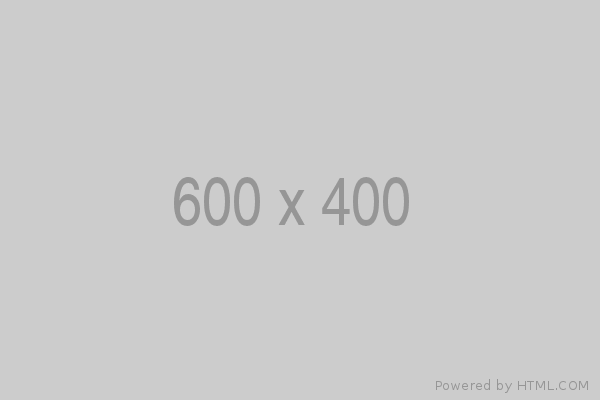
\includegraphics[width=0.5\textwidth]{images/placeholder.png}
    \caption{Pontos decorados que são detectados pela medida aplicada no retângulo R.}
    \label{fig:dec_rect}
\end{figure}

\begin{defi}
    Seja $R=[a,b]\times [c,d]$, em que $a < b \leq c < d$ e considere o ponto decorado $(p^*, q^*)$ com $p^* < q^*$.
    Definimos $(p^*, q^*) \in R$ se alguma das condições equivalentes é verdade:
    \begin{itemize}
        \item Se $p^* \in [a,b]$ e $q^* \in [c,d]$;
        \item Se $a < p^* < b$ e $c < q^* < d$ na ordem total definida anteriormente;
        \item Se $a^+ \leq p^* \leq b^-$ e $c^+ \leq q^* \leq d^-$;
        \item Se o intervalo satisfaz: $[b,c] \subseteq (p^*, q^*) \subseteq (a,d)$;
        \item O ponto com o traço $(p^*, q^*)$ está dentro do retângulo $R$.
    \end{itemize} 
\end{defi}

\begin{defi}
    Definimos com o \textbf{r-interior} do retângulo $R$ o conjunto
    \begin{equation*}
        R^\times = \Set{(p^*, q^*) | (p^*, q^*) \in R}.
    \end{equation*} 
    Também podemos definir o \textbf{interior} de $R$ como o conjunto
    \begin{equation*}
        R^\circ = (a,b) \times (c,d).
    \end{equation*}
\end{defi}

A expressão $|_R$ indica a restrição de um multiconjunto de pontos decorados no retângulo $R$.

\begin{cor}
    Suponha que $\mathfrak{V}$ seja um módulo de persistência decomponível sobre $R$.
    \begin{equation*}
        \mathfrak{V} = \bigoplus_{l \in L} k(p^*_l, q^*_l).
    \end{equation*}
    Então 
    \begin{equation*}
        \mu_{\mathfrak{R}}(R) = \text{card}(\text{Dgm}(\mathfrak{V}\left.)\right|_R)
    \end{equation*}
    para todo retângulo $R = [a,b] \times [c,d]$ com $a < b \leq c < d$. 
\end{cor}
\begin{proof}
   A demonstração segue direto das Proposições \ref{teo:int_meas} e \ref{teo:direct_sum}. 
\end{proof}

A função $\mu$ é chamada de medida pois é aditiva em relação a divisão dos retângulos. 
Vamos provar este fato agora.

\begin{propo}\label{teo:split_measure}
    $\mu_{\mathfrak{V}}$ é aditiva sobre divisão vertical e horizontal dos retângulos:
    \begin{align*}
        \mu_{\mathfrak{V}}([a,b]\times[c,d]) = \mu_{\mathfrak{V}}([a,p]\times[c,d]) 
        + \mu_{\frakv}([p,b] \times [c,d]) \\
        \mu_{\mathfrak{V}}([a,b]\times[c,d]) = \mu_{\mathfrak{V}}([a,b]\times[c,q]) 
        + \mu_{\frakv}([a,b] \times [q,d])
    \end{align*}
    para todo $a < p < b \leq c < q < d$. Esta propriedade pode ser visualizada na Figura 
    \ref{fig:split_measure}.
    \begin{figure}[htpb!]
        \centering
        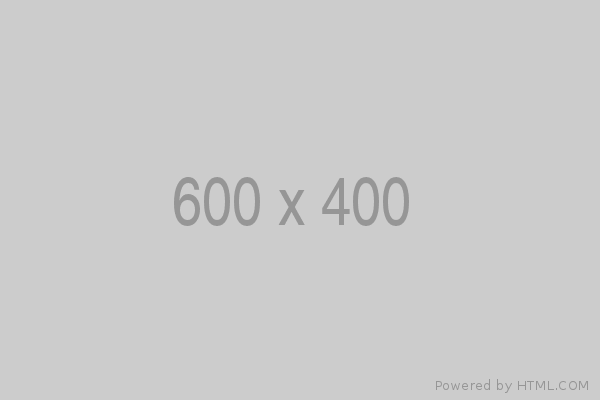
\includegraphics[width=0.5\textwidth]{images/placeholder.png}
        \caption{Representação gráfica da Proposição \ref{teo:split_measure}}
        \label{fig:split_measure}
    \end{figure}
\end{propo}
\begin{proof}
    A demonstração segue direto da Proposição~\ref{teo:restr_princ}: para a aditividade na divisão
    horizontal temos que
    \begin{align*}
        \mu_{\frakv}([a,b] \times [c,d]) & = \innerproduct{\qoff{a} \qem \qno \qem \qon{b} \qem \qon{c} \qem \qoff{d}} \\
        &=\innerproduct{\qoff{a} \qem \qon{p} \qem \qon{b} \qem \qon{c} \qem \qoff{d}}
          + \innerproduct{\qoff{a} \qem \qoff{p} \qem \qon{b} \qem \qon{c} \qem \qoff{d}} \\
        &=\innerproduct{\qoff{a} \qem \qon{p} \qem \qno \qem \qon{c} \qem \qoff{d}}
          + \innerproduct{\qno \qem \qoff{p} \qem \qon{b} \qem \qon{c} \qem \qoff{d}} \\
        &=\mu_{\frakv}([a,p] \times [c,d]) + \mu_{\frakv}([p,b] \times [c,d]).
    \end{align*}
    De forma análoga vale o resultado para a divisão vertical.  
\end{proof}

\subsection{r-medidas abstratas}
Até agora trabalhamos com módulos de persistência e uma medida associada. Porém, podemos
trabalhar de forma mais abstrata, sem mencionar os módulos. 

\begin{defi}
    Seja $\mathcal{D} \subseteq \mathbb{R}^2$. Defina
    \begin{equation*}
        \text{Rect}(\mathcal{D}) = \Set{[a,b]\times[c,d] \subset \mathcal{D} | a < b \text{ e } c < d}.  
    \end{equation*} 
    A \textbf{r-medida} ou \textbf{medida retangular} em $\mathcal{D}$ é uma função
    \begin{equation*}
        \mu \colon \text{Rect}(\mathcal{D}) \to \Set{0,1,\dots} \cup \Set{\infty},
    \end{equation*}
    que também é aditiva na divisão horizontal e vertical dos retângulos. 
\end{defi}

\begin{propo}
    Seja $\mu$ uma \textbf{r-medida} em $\mathcal \subseteq \mathbb{R}^2$. Então 
    \begin{itemize}
        \item Se $R \in \text{Rect}(\mathcal{D})$ pode ser escrito como a união de retângulos com interior
        disjuntos, $R = R_1 \cup \dots \cup R_n$, então $\mu(R) = \sum \mu(R_i)$;
        \item Se $R \subseteq S$, então $\mu(R) \leq \mu(S)$.
    \end{itemize}    
\end{propo}
\begin{proof}
    (\textit{Finitamente aditiva}) Seja $R = [a,b] \times [c,d]$. Por indução e pela propriedade de divisão
    vertical, temos que a aditividade finita vale para decomposições da forma 
    \begin{equation*}
        R = \bigcup_i R_i,
    \end{equation*}
    em que cada $R_i = [a_i, a_{i+1}] \times [c,d]$, com $a = a_1 < \dots < a_m = b$. De forma análoga,
    vale para divisões horizontais e portanto a aditividade vale para decomposições da forma
    \begin{equation*}
        R = [a,b] \times [c,d] = \bigcup_{i,j} R_{ij},
    \end{equation*}
    onde $R_{ij} = [a_i, a_{i+1}] \times [c_j, c_{j+1}]$ com $a = a_1 < \dots < a_m = b$ e $c = c_1 < 
    \dots < c_n = d$. Para uma decomposição arbitrária $R = R_1 \cup \dots \cup R_k$ o resultado segue
    considerando uma decomposição em que cada $R_i$ é decomposto em intervalos da forma acima.  

    (\textit{Monotonicidade}) Decomponha $S$ em uma coleção de retângulos $R$ e $R_1, \dots, R_k$ que 
    possuem interiores disjuntos. Portanto, da propriedade de aditividade e que $\mu \geq 0$
    \begin{align*}
        \mu(S) & = \mu(R) + \mu(R_1) + \dots + \mu(R_k) \\
               & \geq \mu(R).
    \end{align*}
\end{proof}

\begin{propo}{(Subaditividade)} 
    Seja $\mu$ uma \textbf{r-medida} em $\mathcal{D} \subseteq \mathbb{R}^2$. Se um retângulo $R \in 
    \text{Rect}(\mathcal{D})$ está contido numa união finita de retângulos $R_i \in \text{Rect}(
    \mathcal{D})$
    \begin{equation*}
        R \subseteq R_1 \cup \dots \cup R_k,
    \end{equation*}
    então
    \begin{equation*}
        \mu(R) \leq \mu(R_1) + \dots + \mu(R_k).
    \end{equation*}
\end{propo}
\begin{proof}
    Seja $a_1 < \dots < a_m$ sequência de todos os valores do eixo $x$ de cada vértice dos retângulos. 
    Considere também $c_1 < \dots < c_n$ sequência de todos os valores do eixo $y$ de cada vértice dos retângulos.
    Então cada retângulo $R_k$ pode ser decomposto como união dos seguintes subretângulos
    \begin{equation*}
        [a_i, a_{i+1}] \times [c_j, c_{j+1}],
    \end{equation*}
    que possuem interiores disjuntos por construção e sua medida é a soma das medidas de cada subretângulo. 
    Como cada subretângulo de $R$ pertence a um ou mais retângulos $R_i$, segue da aditividade o resultado.
    A Figura~\ref{fig:dem_subadd} mostra uma demonstração visual desta proposição. 
    \begin{figure}[htpb!]
        \centering
        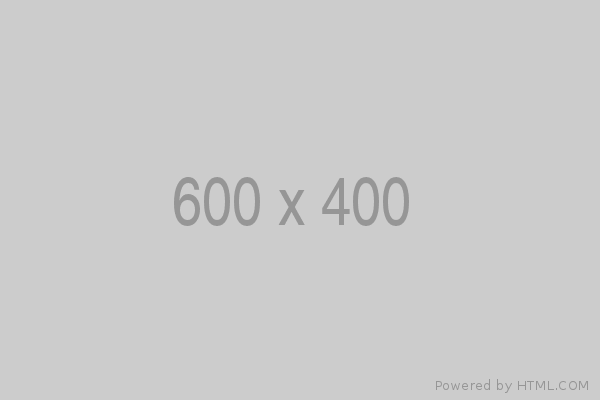
\includegraphics[width=0.7\textwidth]{images/placeholder.png}
        \caption{Demonstração da proposição através da figura.}
        \label{fig:dem_subadd}
    \end{figure}
\end{proof}

\subsection{Equivalência de medidas e diagramas}
As $r$-medidas de persistência permitem o estudo dos diagramas de persistência de maneira mais analítica,
facilitando o desenvolvimento da teoria. Nesta seção iremos demonstrar a equivalência entre medidas 
abstratas e multiconjuntos localmente finitos. Para isso, assumiremos que a medida é finita, como dito
anteriormente. 

O \textbf{$r$-interior} de uma região $\mathcal{D} \subseteq \mathbb{R}^2$ é o conjunto definido abaixo
\begin{equation*}
    \mathcal{D}^\times = \Set{(p^*, q^*) | \exists R \in \text{Rect}(\mathcal{D}) \text{ tal que }
    (p^*, q^*) \in R}.
\end{equation*}
A definição acima pode ser vista com o seguinte significado: o conjunto dos ponto decorados pode ser 
determinado por algum retâgulo em $\mathcal{D}$. 

O \textbf{interior} de $\mathcal{D}$ é dado por 
\begin{equation*}
    \mathcal{D}^\circ = \Set{(p,q) | \exists R \in \text{Rect}(\mathcal{D}) \text{ tal que } 
    (p,q) \in R^\circ},
\end{equation*}
onde para um retângulo $R = [a,b]\times[c,d]$, $R^\circ = (a,b)\times(c,d)$. 

\begin{teo}{(O teorema da equivalência)}\label{teo:equiv_meas}
    Seja $\mathcal{D} \subseteq \mathbb{R}^2$. Então existe uma correspondência bijetiva
    entre
    \begin{enumerate}
        \item $r$-medidas $\mu$ finitas em $\mathcal{D}$. Finito neste caso significa que 
        $\mu(R) < \infty$ para todo $R \in \text{Rect}(\mathcal{D})$.
        \item Multiconjuntos $A$ em $\mathcal{D}$ localmente finitos. Localmente finito significa
        $\text{card}(\left.A\right|_R) < \infty$ para todo $R \in \text{Rect}(\mathcal{D})$.
    \end{enumerate}
    A medida $\mu$ correspondente ao multiconjunto $A$ é relacionada pela fórmula
    \begin{equation}\label{eq:med_dgm}
        \mu(R) = \text{card}(\left.A\right|_R)
    \end{equation}
    para todo $R \in \text{Rect}(\mathcal{D})$, ou equivalentemente
    \begin{equation}\label{eq:med_mult}
        \mu(R) = \sum_{(p^*,q^*)\in R} m(p^*, q^*),
    \end{equation}
    em que
    \begin{equation*}
        m \colon \mathcal{D}^{\times} \to \Set{0,1,2,\dots}
    \end{equation*}
    é a função multiplicidade de $A$. 
\end{teo}
\begin{proof}
$(2) \to (1):$ para este passo, basta provar que a medida definida na Eq. \eqref{eq:med_dgm} é uma $r$-medida.
De fato, é finita pois $A$ é localmente finito. Para verificar a aditivade, suponha que para um retângulo
$R$ qualquer, ele se divida horizontalmente ou verticalmente em $R_1$ e $R_2$. Note então que $(p^*,q^*)$
pertence a exatamente $R_1$ ou $R_2$. Portanto, 
\begin{equation*}
    \mu(R) = \text{card}(\left.A\right|_R) = \text{card}(\left.A\right|_{R_1}) + \text{card}(\left.A\right|_{R_2})
     = \mu(R_1) + \mu(R_2),
\end{equation*}
provando a primeira implicação. 

\noindent$(1) \to (2):$ Dada uma $r$-medida, iremos (1) construir o multiconjunto $A$ em $\mathcal{D}^\times$,
(2) mostrar que $\mu$ e $A$ estão relacionadas pela Eq. \eqref{eq:med_dgm} e (3) mostrar que $A$ é único. Na 
prática, iremos construir a função de multiplicidade $m$ e definir a Eq. \eqref{eq:med_mult} ao invés de $A$ diretamente.

\textbf{Passo 1.} (Fórmula da multiplicidade) Seja $\mu$ uma $r$-medida finita em $\mathcal{D}$. Define
\begin{equation}
    m(p^*, q^*) = \min \Set{\mu(R) | R \in \text{Rect}(\mathcal{D}), (p^*, q^*) \in R}
\end{equation}  
para $(p^*, q^*) \in \mathcal{D}^\times$. Observe que o mínimo é atingido, já que tomamos $(p^*, q^*) \in \mathcal{D}^\times$
e $\mu$ é uma medida que assume valores inteiros. Utilizaremos uma definição alternativa, ao invés de minimizar sob 
todos os retângulos, tomamos o limite de uma sequência de retângulos decrescentes.  
\begin{lema}\label{teo:lem_med}
    Sejam $(\xi_i)$ e $(\eta_i)$ duas sequências não crescentes de números reais positivos
    que tendem a zero quando $i \to \infty$. Então
    \begin{equation*}
        m(p^+, q^+) = \lim_{i\to\infty} \mu([p,p+\xi_i] \times [q, q+\eta_i]),
    \end{equation*}
    e similarmente
    \begin{align*}
        & m(p^+, q^-) = \lim_{i\to\infty} \mu([p,p+\xi_i] \times [q-\eta_i, q]), \\
        & m(p^-, q^+) = \lim_{i\to\infty} \mu([p-\xi_i,p] \times [q, q+\eta_i]), \\
        & m(p^-, q^-) = \lim_{i\to\infty} \mu([p-\xi_i,p] \times [q-\eta_i,q]).
    \end{align*}
\end{lema}
\begin{proof}
    Note primeiro que a sequêncina de retângulos $R_i = [p, p+\xi_i] \times [q, q+\eta_i]$ é 
    cofinal no conjunto de retângulos $R$ contendo $(p^+, q^+)$, ou seja, para todo $R$ deste 
    tipo, $R_i \subseteq R$ para $i$ suficientemente grande.
    
    Pela monotonicidade de $\mu$ e como a sequência de inteiros não negativos $\mu(R_i)$ é não 
    crescente, ela estabiliza no seu limite em algum momento. Portanto
    \begin{equation*}
        m(p^+, q^+) \leq \min_i\mu(R_i) = \lim_{i\to\infty} \mu(R_i) \leq \mu(R)
    \end{equation*}
    para todo $R$ contendo $(p^+, q^+)$. Tomando o mínimo de ambos os lados da inequalidade acima 
    sob todos os $R$, o lado direito se torna $m(p^+, q^+)$, logo
    \begin{equation*}
        m(p^+, q^+) = \lim_{i\to\infty}\mu(R_i).
    \end{equation*}
    Os outros três casos são similares. 
\end{proof} 

\textbf{Passo 2.} Uma vez com a função multiplicidade definida, mostraremos que ela está de acordo com a 
Eq. \eqref{eq:med_mult}. Podemos definir uma medida baseada na função multiplicidade
\begin{equation*}
    \nu(R) = \sum_{(p^*, q^*)\in R} m(p^*, q^*),
\end{equation*}
nos resta mostrar então que $\mu = \nu$. Vamos utilizar indução sobre $k = \mu(R)$. 

\noindent \textbf{Caso base.} Se $\mu(R) = 0$, então para todo $(p^*, q^*) \in R$ temos 
\begin{equation*}
    0 \leq m(p^*, q^*) \leq \mu(R) = 0.
\end{equation*}
Portanto, $\nu(R) = 0$. 

\noindent \textbf{Passo indutivo.} Suponha qe $\mu(R) = \nu(R)$ para todo retângulo $R$ com 
$\mu(R) < k$. Seja agora um retângulo $R_0$ tal que $\mu(R_0) = k$. Vamos mostrar que $\nu(R_0)
=0$. A ideia para este passo é em construir uma sequência decrescente de retângulos fechados 
de forma que haverá apenas um ponto na interseção destes retângulos (Teorema de Cantor). 

Divida o retângulo em quatro quadrantes iguais, $S_1, \dots, S_4$. Pela aditividade finita
\begin{align*}
    \mu(R_0) & = \mu(S_1) + \dots + \mu(S_4) \\
    \nu(R_0) & = \nu(S_1) + \dots + \nu(S_4).
\end{align*}
Se todo quadrante satisfaz $\mu(S_i) < k$, segue então que $\mu(R_0) = \nu(R_0)$, concluindo
a demonstração. Caso contrário, um dos quadrantes tem valor $k$, enquanto o resto será $0$. 
Seja $R_1$ o quadrado especial, então $\mu(R_1) = k$. Resta mostrar que $\nu(R_1) = k$. 

Repetindo o argumento acima, divida o retângulo $R_i$ em quatro quadrantes iguais. Temos dois
casos: todos os quadrantes satisfazem a hipótese indutiva $\mu<k$ e teriamos terminado a situação.
Ou existe um quadrante $R_{i+1}$ com $\mu(R_{i+1})=k$ e temos que mostrar que $\nu(R_{i+1})$.

No pior caso, temos uma sequência decrescente de retângulos fechados
\begin{equation*}
    R_0 \supset R_1 \supset R_2 \supset \dots
\end{equation*}
com cada quadrante sendo do mesmo tipo anterior, $\mu(R_i) = k$. Pelo teorema de cantor e o fato
que o diâmetro dos conjuntos tende a $0$, temos que a interseção dos intervalos fechados possuem
apenas um ponto $(r,s)$.

Vamos mostrar agora que $\nu(R_0) = k$ avaliando a soma explicitamente sob todos os pontos decorados
em $R_0$.

Note primeiro que pontos decorados em $R_0$ que saem da sequência de retângulos em algum momento não
contribuem para $\nu(R_0)$, já que se $(p^*, q^*) \in R_0$ e $(p^*, q^*) \in R_{i-1} - R_i$ para 
algum $i$, então o ponto pertence a algum dos outros três quadrantes, sendo assim $\mu = 0$. 
Portanto, pela fórmula de multiplicidade, $m(p^*, q^*) = 0$. 

Assim, os únicos pontos que contribuem para $\nu(R_0)$ são as variações decoradas de $(r,s)$, já 
que é o único ponto não decorado na interseção. Agora a avaliação de $\nu(R_0)$ depende de como 
este ponto decorado se encontra na intereseção. Existem 3 possíveis casos: as 4, 2, 1 decorações
estão contidas nos retângulos, como podemos ver na Figura \ref{fig:proof_rect}

\begin{figure}[htpb!]
    \centering
    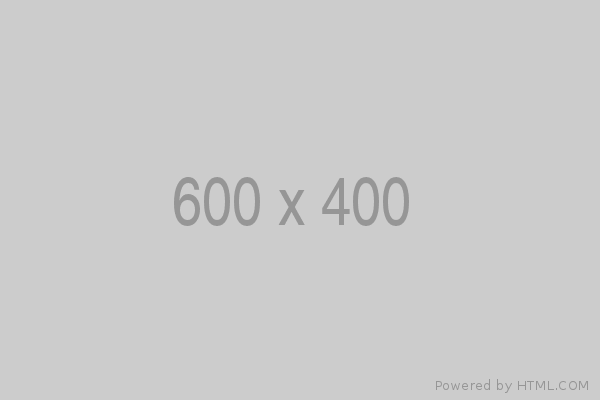
\includegraphics[width=0.7\textwidth]{images/placeholder.png}
    \caption{Possíveis casos dos pontos decorados $(r^*, s^*)$ na interseção $\cap_i R_i$.}
    \label{fig:proof_rect}
\end{figure}

Vamos mostrar apenas para o caso em que as 4 decorações estão em todos os retângulos $R_i$. Os outros
dois casos são análogos. 

Suponha que todas as decorações $(r^*, s^*) \in R_i$ para todo $i$. Agora divida cada retângulo
$R_i$ em quatro partes, de forma que cada parte contenha apenas uma decoração: $R_i^{++}, R_i^{+-},
R_i^{-+}, R_i^{--}$. A divisão ocorre de forma que o ponto $(r,s)$ fique num vértice dividido pelos 
quatro retângulos. Pelo Lema \ref{teo:lem_med},
\begin{align*} 
    & m(r^+, s^+) = \lim_{i \to \infty} \mu(R_i^{++}), \quad m(r^+, s^-) = \lim_{i \to \infty} \mu(R_i^{+-}), \\
    & m(r^-, s^+) = \lim_{i \to \infty} \mu(R_i^{-+}), \quad m(r^-, s^-) = \lim_{i \to \infty} \mu(R_i^{--}).
\end{align*}
Além disso, cada uma dessas sequências decrescentes de inteiros estabilizam no seu limite. Portanto, para valores
de $i$ suficientemente grandes
\begin{align*}
    \nu(R_0) & = m(r^+, s^+) + m(r^+, s^-) + m(r^-, s^+) + m(r^-, s^-) \\
             & = \mu(R_i^{++}) +  \mu(R_i^{+-}) + \mu(R_i^{-+}) + \mu(R_i^{--}) = \mu(R_i) = k. 
\end{align*}

\textbf{Passo 3.} (Unicidade) Suponha que $m'(p^*, q^*)$ é um outra função multiplicidade em $\mathcal{D}^\times$ 
cuja $r$-medida associada 
\begin{equation*}
    \nu'(R) = \sum_{(p^*, q^*) \in R} m'(p^*, q^*)
\end{equation*}
satisfaz $\mu = \nu'$. Vamos mostrar que $m=m'$. 

Seja $(p^*, q^*) \in \mathcal{D}^\times$ e $R$ um retângulo que contém o ponto $(p^*, q^*)$ em um
dos seus vértices. Como $\nu(R) = \nu'(R) = \mu(R) < \infty$, existem apenas finitos pontos decorados
em $R$. Além disso, podemos diminuir $R$ de forma que $(p^*, q^*)$ seja o único ponto decorado em $R$
com multiplicidade positiva em ambas as medidas. Portanto,
\begin{equation*}
    m(p^*, q^*) = \nu(R) = \mu(R) = \nu'(R) = m'(p^*, q^*).
\end{equation*} 
Como $(p^*, q^*)$ era um ponto qualquer, segue o resultado. 
\end{proof}

\begin{defi} 
    Seja $\mu$ uma medida finita em $\mathcal{D} \subseteq \mathbb{R}^2$. Então
    \begin{itemize}
        \item o \textbf{diagrama decorado} de $\mu$ é o único multiconjunto localmente finito
        $\text{Dgm}(\mu)$ em $\mathcal{D}^{\times}$ tal que 
        \begin{equation*}
            \mu(R) = \text{card}(\text{Dgm}(\mu\left.)\right|_R)
        \end{equation*}
        para todo retângulo $R \in \text{Rect}(\mathcal{D})$;
        \item o \textbf{diagrama não decorado} de $\mu$ é o multiconjunto localmente finito em 
        $\mathcal{D}^{\circ}$
        \begin{equation*}
            \text{dgm}(\mu) = \Set{(p,q) | (p^*, q^*) \in \text{Dgm}(\mu)} \cap \mathcal{D}^\times 
        \end{equation*}
        obtido esquecendo a decoração dos pontos e restringindo ao interior. 
    \end{itemize}
\end{defi}

\section{Comportamento de módulos e exemplos}

Quando extende-se as medidas e diagramas de persistência para o semiplano diagonal superior com os 
pontos no infinito e para medidas que assumem valor infinito também, os módulos de persistência não são
sempre bem comportados, necessitando diferenciar entre as diversas situações.
Abaixo estão três diferentes noções e em seguida apresentaremos apenas mais uma, já que estamos trabalhando
apenas com medidas finitas. 

\begin{itemize}
    \item Um módulo de persistência é do \textbf{tipo finito} se é uma soma direta finita de módulos intervalares;
    \item Um módulo de persistência é \textbf{localmente finito} se é uma soma direta de módulos intervalares
    e satisfaz a seguinte propriedade: qualquer subconjunto de $\mathbb{R}$ intersecta um número finito de 
    módulos intervalares;
    \item Um módulo de persistência $\frakv$ é \textbf{pontualmente de dimensão finita (pfd)} se cada espaço
    vetorial $V_t$ tiver dimensão finita. 
\end{itemize}

Como estamos trabalhando medidas finitas apenas, vamos definir o módulo \textit{q-tame}. Seja 
$\frakv$ um módulo de persistência. Dizemos que $\mathfrak{V}$ é \textit{q-tame} se 
$\mu_{\frakv}(Q) < \infty$ para todo quadrante $Q$ que não toca a diagonal. Em outras palavras
\begin{equation*}
    \innerproduct{\qon{b} \qem \qon{c} \mid \frakv} < \infty
\end{equation*}
para todo $b < c$. O diagrama de persistência $\text{Dgm}(\mu_\frakv)$ é definido sobre o conjunto
\begin{equation*}
    \Set{(p^*, q^*) | -\infty \leq p < q \leq + \infty}.
\end{equation*}

Abaixo mostramos alguns exemplos que encontra-se na teoria para módulos de persistência \textit{q-tame}.

\begin{teo}\label{teo:tameum}
Seja $X$ um poliedro compacto e $f \colon X \to \mathbb{R}$ uma função contínua. Então a homologia
persistente $H(\mathfrak{X}_{\text{sub}})$ da filtração de subnível de $(X,f)$ é \textit{q-tame}. 
\end{teo}
\begin{proof}
Precisamos mostrar que 
\begin{equation*}
    H(X^b) \to H(X^c) 
\end{equation*}
tem rank finito para qualquer $b < c$. Considere uma triangulação de $X$ e a subdivida de forma que 
nenhum simplexo intersecte $f^{-1}(b)$ e $f^{-1}(c)$ ao mesmo tempo. Defina agora $Y$ como a união
de todos os simplexos que intersectam $X^b$. Portanto, 
\begin{equation*}
    X^b \subseteq Y \subseteq X^c
\end{equation*} 
e aplicando o funtor de homologia
\begin{equation*}
    H(X^b) \longrightarrow H(Y) \longrightarrow H(X^c).
\end{equation*}
Como $Y$ é um poliedro compacto, $H(Y)$ tem dimensão finita, portanto a aplicação $H(X^b) \to H(X^c)$ 
tem rank finito. 
\end{proof}

\begin{cor}\label{teo:tamedois}
Seja $X$ um poliedro localmente compacto e $f \colon X \to \mathbb{R}$ uma função propriamente contínua
que seja limitada por baixo. Então $H(\mathfrak{X}_{\text{sub}})$ é \textit{q-tame}.
\end{cor}
\begin{proof}
Novamente, precisamos mostrar que $H(X^b) \to H(X^c)$ tem rank finito. Mas neste caso iremos aplicar
o Teorema~\ref{teo:tameum}, para tanto precisamos de um subpoliedro compacto de $X$ que contenha $X^c$. 
Seja uma triangulação local finita de $X$ e considere os simplexos fechados que intersectam $X^c$. 
Como $X^c$ é compacto, já que $f$ é uma função própria, no sentido que a pre-imagem de compacto é compacto,
temos que existe um número finito de conjuntos fechados que intersecta $X^c$. Considere agora a união
desses conjuntos fechados como o subpoliedro desejado. 
\end{proof}

\begin{cor}\label{teo:tametres} 
Seja $A$ um subconjunto não vazio compacto de $X = \mathbb{R}^n$ e $f \colon X \to \mathbb{R}$, $f(x) =
\min_{a\in A} \norm{x-a}$, para qualquer norma $\norm{.}$. Segue então do Corolário \ref{teo:tamedois}
que $H(\mathfrak{X}_{\text{sub}})$ é \textit{q-tame}.
\end{cor}

\section{\textit{Intercalação}} 

A intercalação é um modo de comparar dois módulos de persistência. Dizemos que os módulos
$\mathfrak{U}$ e $\frakv$ são isomorfos se existem homomorfismos
\begin{equation*}
    \Psi \in \text{Hom}(\mathfrak{U}, \frakv), \quad \Phi \in \text{Hom}(\frakv, \fraku), 
\end{equation*}
tais que 
\begin{equation*}
    \Psi \Phi = 1_\fraku, \quad \Phi \Psi = 1_\frakv.
\end{equation*}

No entanto, para trabalhar com módulos de persistência, a noção de isomorfismo é muito forte. 
Para isso, podemos enfraquece-la definindo a $\delta$-intercalação entre dois módulos. 
Nesta subseção iremos definir o interlaçamento e demonstrar o lema de interpolação,
como se define um \textit{caminho contínuo} entre dois módulos de persistência. 

\subsection{Homomorfismos e módulos de persistência}

Primeiro vamos considerar homomorfismo que mudam o índice de persistência dos módulos. 
Sejam $\fraku, \frakv$ módulos de persistência sobre $\mathbb{R}$ e $\delta \in \mathbb{R}$
qualquer. Então um homomorfismo de grau $\delta$ é a coleção $\Phi$ de aplicações lineares
\begin{equation*}
    \phi_t \colon U_t \to V_{t+\delta}
\end{equation*}
para todo $t \in \mathbb{R}$ tal que o diagrama 
\begin{equation*}
    \begin{tikzcd}[row sep=huge, column sep = huge]
        & U_s \rar{u_t^s} \dar[swap]{\phi_s} & U_t \dar{\phi_t} \\
        & V_{s+\delta} \rar{v^{s+\delta}_{t+\delta}} & V_{t+\delta}
    \end{tikzcd}
\end{equation*}
comuta para todo $s \leq t$. Escrevemos 
\begin{align*}
    \text{Hom}^\delta(\mathfrak{U}, \mathfrak{V}) &= \Set{\text{homomorfismos } \mathfrak{U} \to \mathfrak{V}}
    \text{ de grau } \delta, \\
    \text{End}(\mathfrak{V}) &= \Set{\text{homomorfismos } \mathfrak{V} \to \mathfrak{V}\text{ de grau } \delta}.
\end{align*}
A composição é definida de forma natural, nos dando a aplicação
\begin{equation*}
    \text{Hom}^{\delta_2}(\frakv, \mathfrak{W}) \times \text{Hom}^{\delta_1}(\fraku, \frakv) 
    \to \text{Hom}^{\delta_1 + \delta_2}(\fraku, \mathfrak{W}).
\end{equation*}
Para $\delta \geq 0$, a aplicação de grau $\delta$ mais importante é a aplicação
\textit{shift}
\begin{equation*}
    1^\delta_\frakv \in\text{End}^\delta(\frakv),
\end{equation*}
que é a coleção de aplicações lineares $(v_{t+\delta}^t)$ da estrutura de $\frakv$. Se $\Phi$ 
é um homomorfismo $\fraku \to \frakv$ de grau quaqluer, então por definição 
\begin{equation*}
    \Phi 1_\fraku^\delta = 1_\fraku^\delta \Phi,
\end{equation*}
para todo $\delta \geq 0$. 

\begin{obs}
Podemos escrever os morfismos de grau não nulos de forma diferente. Seja $\frakv$ um módulo
de persistência e $\delta \in \mathbb{R}$ qualquer, denotamos por $\frakv[\delta]$ o 
\textbf{módulo transladado} 
\begin{equation*}
    (V[\delta])_t = V_{t+\delta}, \qquad (v[\delta])^s_t = v^{s+\delta}_{t+\delta},
\end{equation*}
ou seja, $V[\delta]$ é o módulo $\frakv$ transladado em $\delta$ para baixo. Além disso,
temos identificações com os homomorfismos
\begin{equation*}
    \text{Hom}^\delta(\fraku, \frakv) = \text{Hom}(\fraku, \frakv[\delta]) 
    = \text{Hom}(\fraku[a], \frakv[a+\delta])
\end{equation*}
para todo $a \in \mathbb{R}$. 
\end{obs}

\begin{defi}
    Seja $\delta \geq 0$. Dizemos que $\fraku, \frakv$ são $\delta$-interlaçados se
    existem aplicações 
    \begin{equation*}
        \Phi \in \Hom^\delta(\fraku, \frakv), \Psi \in \Hom^\delta(\frakv, \fraku) 
    \end{equation*}
    tais que
    \begin{equation*}
        \Psi\Phi = 1_\fraku^{2\delta}, \Phi\Psi = 1_\frakv^{2\delta}.
    \end{equation*}
\end{defi}

\begin{ex}
    Seja $X$ um espaço topológico e $f,g \colon X \to \mathbb{R}$. Suponha que $\norm{f-g}_\infty 
    < \delta$. Então os módulos de persistência $H(\mathfrak{X}^f_{\text{sub}}), H(\mathfrak{X}^g_{\text{sub}})$
    são $\delta$-interlaçados.  
    
    De fato, note primeiro que 
    \begin{align*}
        & (X,f)^t \subseteq (X,g)^{t+\delta} \\
        & (X,g)^t \subseteq (X,f)^{t+\delta},
    \end{align*}
    já que para $x \in (X,f)^t$ temos que $f(x) \leq t$ e como 
    $\norm{f-g}_\infty < \delta$, $\abs{g(x) - f(x)} < \delta$ 
    e logo $g(x) < f(x) + \delta \leq t + \delta$, implicando 
    $x \in (X,g)^{t+\delta}$. De forma análoga temos a segunda equação.  

    Pela funtorialidade de $H$, temos que para todo $t$, existem aplicações lineares induzidas das
    inclusões acima
    \begin{align*}
        \Phi \colon H(\mathfrak{X}_{\text{sub}}^f) \to H(\mathfrak{X}_{\text{sub}}^g) \\
        \Psi \colon H(\mathfrak{X}_{\text{sub}}^g) \to H(\mathfrak{X}_{\text{sub}}^f)
    \end{align*}
    de grau $\delta$. Como as aplicações são decorrentes de um funtor, as condições de interlaçamento
    são satisfeitas.
\end{ex}

Da mesma forma que módulos de persistência podem ser vistos sobre posets, uma relação de 
interlaçamento entre dois módulos pode ser vista como um módulo de persistência sobre um poset. A seguir
iremos desenvolver esta ideia. 

Considere a seguinte ordem parcial no plano
\begin{equation*}
    (p_1, q_1) \leq (p_2, q_2) \iff p_1 \leq p_2, q_1 \leq q_2.
\end{equation*}
Agora, para todo número real $x$, defina a faixa diagonal transladada no plano
\begin{equation}\label{eq:iso_delta}
    \Delta_x = \Set{(p,q) | q-p = 2x} = \Set{(t-x, t+x) | t \in \mathbb{R}}.
\end{equation}
$\Delta_x$ visto como um poset é isomorfo à reta real. Iremos usar o isomorfismo de
\eqref{eq:iso_delta} como uma identificação canônica entre módulos de persistência
sobre $\mathbb{R}$ e sobre $\Delta_x$. 

\begin{propo}\label{teo:prop_inter}
Sejam $x,y$ números reais. Os módulos de persistência $\mathfrak{U}$ 
e $\frakv$ são $\abs{y-x}$-intercalados se, e somente se, existe 
um módulo de persistência $\mathfrak{W}$ sobre $\Delta_x \cup
\Delta_y$ tal que $\left.\mathfrak{W}\right|_{\Delta_x} = 
\mathfrak{U}$ e  $\left.\mathfrak{W}\right|_{\Delta_y} = 
\mathfrak{V}$. O conjunto $\Delta_x \cup \Delta_y$ é um subposet
de $\mathbb{R}^2$.  
\end{propo}
\begin{proof}

\end{proof}

\subsection{O lema de interpolação}

Vamos anunciar o lema da interpolação, que será utilizado na 
demonstração do teorema da estabilidade dos módulos de persistência.

\begin{lema}{(Lema de interpolação)}\label{teo:lema_interp}
Suponha que $\mathfrak{U}$ e $\frakv$ são módulos de persistência
$\delta$-interlaçados. Então existe uma família de módulos de 
persistência $(\mathfrak{U}_x \mid x \in [0,\delta])$ tais que 
$U_0$ e $U_\delta$ são iguais a $\mathfrak{U}$ e $\frakv$ 
respectivamente e $\mathfrak{U}_x$, $\mathfrak{U}_y$ são 
$\abs{y-x}$-interlaçados para todo $x,y \in [0,\delta]$. Além disso,
se $\mathfrak{U}$ e $\mathfrak{V}$ são \textit{q-tames}, então 
$(\mathfrak{U}_x)$ são \textit{q-tames}.
\end{lema}

O Teorema~\ref{teo:lema_interpdois} é uma versão mais forte do 
Lema~\ref{teo:lema_interp}. 
\begin{teo}{(Lema de interpolação, versão 2)}\label{teo:lema_interpdois}
Todo módulo de persistência sobre $\Delta_0 \cup 
\Delta_\delta, \mathfrak{W}$, se extende a um módulo de persistência 
$\bar{\mathfrak{W}}$ sobre a faixa diagonal
\begin{equation*}
    \Delta_{[0, \delta]} = \Set{(p,q) | 0 \leq q - p \leq 2\delta}
    \subset \mathbb{R}^2.
\end{equation*} 
Se $\left.\mathfrak{W}\right|_{\Delta_0}, \left.\mathfrak{W}
\right|_{\Delta_\delta}$ são \textit{q-tames}, então a extensão
pode ser escolhida de forma que cada $\left.\bar{\mathfrak{W}}
\right|_{\Delta_x}$ é \textit{q-tame}. 
\end{teo}
\begin{proof}
    Sejam $\Delta_0 \cup \Delta_\delta$ e $\Delta_{[0,\delta]}$ duas 
    categorias no mesmo sentido definido no início deste capítulo para
    o conjunto dos reais $\mathbb{R}$ ($s \to t \text{ sss } s \leq t$).
    Então os módulos de persistência sobre esses posets podem ser vistos
    como funtores para a categoria dos espaços vetoriais. O teorema
    de extensão de Kan~\cite{MacLane1978} afirma que existe uma extensão
    $\bar{\mathfrak{W}}$ 
    \begin{equation*}
        \begin{tikzcd}
            {\Delta_{[x_0,x_1]}} \arrow[dotted]{rd}{\bar{\mathfrak{W}}}     &             \\
            \Delta_{x_0} \cup \Delta_{x_1} \arrow{u} \arrow{r}{\mathfrak{W}}  & \text{Vect}
        \end{tikzcd}
    \end{equation*}
    para qualquer funtor $\mathfrak{W}$, completando
    a demonstração. 
\end{proof}

Se $\mathfrak{U}$ e $\frakv$ são $\delta$-interlaçados, então 
pela Proposição~\ref{teo:prop_inter} existe um módulo de 
persistência $\mathfrak{W}$ sobre $\Delta_0 \cup \Delta_\delta$ tal
que $\left.\mathfrak{W}\right|_{\Delta_0} = \mathfrak{U}$ e 
$\left.\mathfrak{W}\right|_{\Delta_\delta} = \frakv$. Pelo 
Teorema~\ref{teo:lema_interpdois}, este módulo se extende a 
$\bar{\mathfrak{W}}$ sobre a faixa $\Delta_{[0,\delta]}$.
Defina então $\mathfrak{U}_x = \left.\bar{\mathfrak{W}}\right|_{
\Delta_x}$, logo $\mathfrak{U}_x$ e $\mathfrak{U}_y$ são 
$\abs{y-x}$-interlaçados para todo $x,y\in [0, \delta]$. 

\section{O teorema de isometria}

Existe uma relação entre os módulos de persistência e seus respectivos diagramas 
de persistência. Para módulos de persistência bem comportados, como os 
\textit{q-tames}, existe uma isometria entre módulos e diagramas. Para mostrar 
parcialmente este resultado, iremos definir a distância de interlaçamento entre
módulos de persistência e também a distância bottleneck, que é calculada
em multiconjuntos. 

\subsection{A distância de interlaçamento}

Para o primeiro passo, iremos definir a distância de interlaçamento entre
módulos de persistência. Primeiro note que para módulos 
$\fraku,  \frakv$ que são $\delta$-interlaçados, então eles
são $(\delta+\epsilon)$-interlaçados para todo $\epsilon > 0$. Basta tomar
os morfismos
\begin{align*}
    & \Phi' = \Phi 1_\fraku^\epsilon = 1_\frakv^\epsilon \Phi \\
    & \Psi' = \Psi 1_\frakv^\epsilon = 1_\fraku^\epsilon \Psi
\end{align*}
que satisfazem a condição de interlaçamento. 

Portanto, o desafio é obter o menor parâmetro possível de forma que módulos
de persistência sejam interlaçados. O problema é que nem sempre é obtido, 
sendo assim definimos o conceito de $\delta^+$-interlaçamento. Dizemos que 
$\fraku, \frakv$ são $\delta^+$-interlaçados se eles são $(\delta + \epsilon)$
-interlaçados para todo $\epsilon > 0$. 

\begin{defi}
    Sejam $\fraku, \frakv$ dois módulos de persistência. A \textbf{distância
    de interlaçamento} entre $\fraku, \frakv$ é dada por
    \begin{align*}
        \di(\fraku, \frakv) &= \inf\Set{\delta | \fraku, \frakv \text{ são }
        \delta \text{-interlaçados}} \\
        &=\min\Set{\delta | \fraku, \frakv \text{ são } \delta^+ 
        \text{-interlaçados}}.
    \end{align*}
    Se não existe nenhum $\delta$-interlaçamento entre $\fraku, \frakv$ para
    qualquer $\delta$, então $\di(\fraku, \frakv) = \infty$.
\end{defi}

\begin{propo}\label{teo:inter_triang}
    A distância de interlaçamento satisfaz a desigualdade triangular:
    \begin{equation*}
        \dt_i(\fraku, \frakw) \leq \dt_i(\fraku, \frakv) + \dt_i(\frakv, \frakw)
    \end{equation*}
    para quaisquer módulos de persistência $\fraku, \frakv$ e $\frakw$. 
\end{propo}
\begin{proof}
    Dados $\delta_1$-interlaçamento entre $\fraku, \frakv$ e $\delta_2$-interlaçamento
    entre $\frakv, \frakw$, então podemos construir um $(\delta_1 + \delta_2)$-
    interlaçamento entre $\fraku, \frakw$ simplesmente compondo as outras duas aplicações
    de interlaçamento
    \begin{align*}
        &\fraku \xrightarrow{\Phi_1} \frakv \xrightarrow{\Phi_2} \frakw \\
        &\fraku \xleftarrow{\Psi_1} \frakw \xleftarrow{\Psi_2} \frakw.
    \end{align*}
    Vamos mostrar que $\Phi = \Phi_2 \Phi_1$ e $\Psi = \Psi_1 \Psi_2$. De fato
    \begin{align*}
        & \Psi\Phi = \Psi_1\Psi_2\Phi_2\Phi_1 = \Psi_1 1^{2\delta_2}_\frakv \Phi_1 
        = \Psi_1\Phi_1 1^{2\delta_2}_\fraku = 1^{\delta_1}_\fraku 1^{\delta_2}_\fraku
        = 1^{2\delta}_\fraku \\
        & \Phi\Psi = \Phi_2\Phi_1\Psi_1\Psi_2 = \Phi_2 1^{2\delta_1}_\frakv \Psi_2 
        = \Phi_2\Psi_2 1^{2\delta_1}_\frakw = 1^{\delta_2}_\frakw 1^{\delta_1}_\frakw
        = 1^{2\delta}_\frakw 
    \end{align*}
    Agora basta tomar o ínfimo entre $\delta_1, \delta_2$.
\end{proof}

A proposição nos diz que $\di$ é uma pseudométrica. Não chega a ser uma métrica, 
pois é possível construir exemplos tais que $\di(\fraku, \frakv) = 0$ não implica
que $\fraku \simeq \frakv$. Só teremos um isomorfismo entre dois módulos \textit{q-tames}
se os diagrams de persistência não decorados forem iguais. 

\begin{ex}
    Os módulos intervalares
    \begin{equation*}
        \kbf[p,q], \kbf[p,q), \kbf(p,q], \kbf(p,q)
    \end{equation*}
    são $0^+$-interlaçados, mas não isomórfos. 
\end{ex}

\begin{propo}\label{teo:direct_sum_dist}
    Sejam $\fraku_1, \fraku_2, \frakv_1, \frakv_2$ módulos de persistência. Então
    \begin{equation*}
        \dt_i(\fraku_1 \oplus \fraku_2, \frakv_1 \oplus \frakv_2) \leq \max(\di(\fraku_1,
        \frakv_1), \di(\fraku_2, \frakv_2)).
    \end{equation*}
    De forma geral a equação acima vale para somas diretas arbitrárias. Sejam $(\fraku_l \mid l \in L)$ 
    e $(\frakv_l \mid l \in L)$ famíias de módulos de persistência indexadas em algum conjunto $L$. Seja
    \begin{equation*}
        \fraku = \bigoplus_{l \in L} \fraku_l, \quad \frakv = \bigoplus_{l \in L} \frakv_l.
    \end{equation*}
    Então
    \begin{equation*}
        \di(\fraku, \frakv) \leq \sup(\di(\fraku_l, \frakv_l) \mid l \in L).
    \end{equation*}
\end{propo}
\begin{proof}
    Dados $\delta$-interlaçamentos $\Phi_l, \Psi_l$ para cada par $\fraku_l, \frakv_l$, as aplicações
    $\Phi = \oplus\Phi_l, \Psi = \oplus \Psi_l$ constituem um $\delta$-interlaçamento entre 
    $\fraku, \frakv$. Portanto, qualquer cota superior de $\di(\fraku_l, \frakv_l)$ é uma cota superior
    de $\di(\fraku, \frakv)$, em particular, para o $\sup$. 
\end{proof}

\subsection{A distância bottleneck}

Com a primeira distância definida, vamos definir a segunda, a bottleneck. Denote por 
\begin{equation*}
    \bar{\mathcal{H}}^\circ = \Set{(p,q) | -\infty \leq p < q \leq +\infty}
\end{equation*}
o semiplano extendido aberto (sem a diagonal). Para definirmos a distância bottleneck,
precisamos definir certas relações entre os pontos em $\hsp$.  
\begin{itemize}
    \item \textbf{ponto a ponto}: A primeira ideia é que dois diagramas não decorados estão
    próximos um do outro se existe uma bijeção entre eles que não leva um ponto muito longe.
    Para definir uma distância entre esses pontos, usamos a métrica $l^\infty$ no plano:
    \begin{equation*}
        \dt^\infty((p,q), (r,s)) = \max(\abs{p-r}, \abs{q-s}).
    \end{equation*}
    Pontos no infinito são calculados da seguinte forma:
    \begin{align*}
        &\dt^\infty((-\infty, q), (-\infty,s)) = \abs{q-s} \\
        &\dt^\infty((p, +\infty), (r,+\infty)) = \abs{p-r} \\
        &\dinf((-\infty, +\infty), (-\infty, +\infty)).
    \end{align*}
    Pontos em regiões diferentes, como $(p,q)$ e $(-\infty,s)$, possuem distância igual a
    $\infty$.
    \item \textbf{ponto a diagonal}: A outra ideia é que pontos próximos da diagonal podem ser
    absorvidos pela diagonal. Usando novamente a métrica $l^\infty$:
    \begin{equation*}
        \dinf((p,q), \Delta) = \frac{1}{2}(q-p).
    \end{equation*}
\end{itemize}

Vamos mostrar agora duas proposições relacionadas com os dois itens acima. 
\begin{propo}\label{teo:int_ineq}
    Sejam $(p^*, q^*)$ e $(r^*, s^*)$ intervalos e 
    \begin{equation*}
        \fraku = \kbfp{p}{q} \text{ e } \frakv = \kbfp{r}{s}
    \end{equation*}
    os módulos intervalares correspondentes. Então
    \begin{equation*}
        \di(\fraku, \frakv) \leq \dt^\infty((p,q), (r,s)).
    \end{equation*}
\end{propo}
\begin{proof}
    A demonstração pode ser encontrada na página $87$ em \cite{Chazal2016}.
\end{proof}

\begin{propo}\label{teo:semint_eq}
    Seja $(p^*, q^*)$ um intervalo e 
    \begin{equation*}
        \fraku = \kbfp{p}{q}
    \end{equation*}
    seu módulo intervalar correspondente. Denote por $0$ o módulo de persistência
    nulo. Então
    \begin{equation*}
        \di(\fraku, 0) = \frac{1}{2}(q-p)
    \end{equation*}
\end{propo}
\begin{proof}
    Seja $\delta \geq 0$. Observe que como tomamos o módulo de persistência nulo, os únicos
    morfismos saindo e chegando nele são os morfismos nulos. Portantno, a única condição
    que precisamos checar é quando dados $\Psi\Phi = 1^{2\delta}_\fraku$, temos 
    $0 = 1^{2\delta}_\fraku$. Isso vale quando $\delta > \frac{1}{2} (q-p)$ e falha 
    para $\delta < \frac{1}{2}(q-p)$. De fato, note que as aplicações $u^t_{t+2\delta} \colon
    U_t \to U_{t+2\delta}$ são nulas precisamente quando $t < p$ ou $t + 2\delta > q$, ou seja,
    $\delta < \frac{1}{2}(q-t)$ e pela primeira condição $(-t > -p)$, teriamos a desigualdade desejada. 
\end{proof}

Utilizando os resultados e definições acima, podemos definir a distância bottleneck entre 
multiconjuntos no semiplano extendido. Neste contexto, iremos adaptar os multiconjuntos 
a conjuntos onde cada elemento possui um índice, ou seja, se $\alpha$ é um elemento de 
multiplicidade $k$, teremos os elementos $\alpha_1, \dots, \alpha_k$. 

\begin{defi}
    Um \textbf{emparelhamento parcial} entre os multiconjuntos $A$ e $B$ é uma coleção de pares
    \begin{equation*}
        M \subset A \times B
    \end{equation*}
    tal que
    \begin{itemize}
        \item para todo $\alpha \in A$ existe no máximo um $\beta \in B$ tal que $(\alpha, \beta)
        \in M$;
        \item para todo $\beta \in B$ existe no máximo um $\alpha \in A$ tal que 
        $(\alpha, \beta) \in M$.
    \end{itemize}
    Além disso, dizemos que um emparelhamento parcial $M$ é um $\delta$-emparelhamento se 
    as seguintes condições são verdadeiras
    \begin{itemize}
        \item se $(\alpha, \beta) \in M$, então $\dinf(\alpha, \beta) \leq \delta$; 
        \item se $\alpha \in A$ não está emparelhado, então $\dinf(\alpha, \Delta) \leq \delta$;
        \item se $\beta \in B$ não está emparelhado, então $\dinf(\beta, \Delta) \leq \delta$.
    \end{itemize}
\end{defi}

\begin{defi}
    A \textbf{distância bottleneck} entre dois multiconjuntos $A,B$ em $\hsp$ é
    \begin{equation*}
        \db(A,B) = \inf \Set{\delta | \text{Existe um } \delta \text{-emparelhamento entre 
        } A \text{ e } B}.
    \end{equation*}
\end{defi}

\begin{propo}
    A distância bottleneck satisfaz a desigualdade triangular
    \begin{equation*}
        \dt_b(A,C) \leq \dt_b(A,B) + \dt_b(B,C)
    \end{equation*}
    para quaisquer multiconjuntos $A, B, C$. 
\end{propo}
\begin{proof}
    Sejam $M_1$ um $\delta_1$-emparelhamento entre $A,B$ e $M_2$ um $\delta_2$-
    emparelhamento entre $B,C$. Defina agora $\delta = \delta_1 + \delta_2$. 
    Vamos definir agora um $\delta$-emparelhamento $M$ entre $A$ e $C$.
    
    Defina $M$ como a composição de $M_1$ e $M_2$, ou seja,
    \begin{equation*}
        M = \Set{(\alpha, \gamma) | \text{Existe um } \beta \in B \text{ tal que }
        (\alpha, \beta) \in M_1 \text{ e } (\beta, \gamma) \in M_2}.
    \end{equation*}
    Observe que $M$ é um emparelhamento parcial pois $M_1, M_2$ são. Resta 
    mostrar agora que $M$ é o $delta$-emparelhamento que procuramos. De fato
    \begin{itemize}
        \item Se $(\alpha, \gamma) \in M$, então
        \begin{equation*}
            \dinf(\alpha, \gamma) \leq \dinf(\alpha, \beta) + \dinf(\beta, \gamma) 
            \leq \delta_1 + \delta_2 = \delta,
        \end{equation*}
        em que $\beta$ é o elemento da definição de $M$ que une $\alpha$ a $\gamma$. 
        \item Se $\alpha$ não está emparelhado em $M$ então há duas possibilidade:
        $\alpha$ não está emparelhado em $M_1$, então por definição
        \begin{equation*}
            \dinf(\alpha, \Delta) \leq \delta_1 \leq \delta,
        \end{equation*}
        e caso $\alpha$ está emparelhado em $M_1$, $(\alpha, \beta) \in M_1$. 
        Portanto, $\beta$ não está emparelhado em $M_2$, caso contrário $\alpha$ estaria 
        emparelhado em $M$. Logo, 
        \begin{equation*}
            \dinf(\alpha, \Delta) \leq \dinf(\alpha, \beta) + \dinf(\beta, \Delta) 
            \leq \delta_1 + \delta_2 = \delta.
        \end{equation*}
        \item Se $\gamma$ não está emparelhado em $M$, de maneira análoga temos que 
        \begin{equation*}
            \dinf(\gamma, \Delta) \leq \delta.
        \end{equation*}
        Assim mostramos que $M$ é o $\delta$-emparelhamento requerido. 
    \end{itemize}
\end{proof}

Por fim, finalizamos a subseção com seu teorema mais importante:
\begin{teo}\label{teo:stb_decom}
    Sejam $\fraku, \frakv$ módulos de persistência decomponíveis. Então 
    \begin{equation*}
        \di(\fraku, \frakv) \leq \dt_b(\dgm{\fraku}, \dgm{\frakv}).
    \end{equation*}
\end{teo}
\begin{proof}
    Vamos mostrar que para todo $\delta$-emparelhamento entre $\dgm{\fraku}$
    e $\dgm{\frakv}$, temos $\di(\fraku, \frakv) \leq \delta$. Após isso 
    tomamos o infimum sobre todo $\delta$ acima e obtemos o resultado. 

    Seja $M$ um $\delta$-emparelhamento entre $\dgm{\fraku}$ e $\dgm{\frakv}$. 
    Como os módulos são decomponíveis, podemos construir $M$ a partir de um
    emparelhamento parcial entre os módulos intervalares de $\fraku$ e $\frakv$.
    
    Reescrevendo $\fraku$ e $\frakv$
    \begin{equation*}
        \fraku = \bigoplus_{l\in L} \fraku_l, \quad \frakv = \bigoplus_{l \in L} \frakv_l
    \end{equation*}
    de forma que cada par é um dos seguintes
    \begin{enumerate}
        \item \label{en:match} um par de intervalos emparelhados;
        \item \label{en:unmatchU} $\fraku_l$ não está emparelhado e $\frakv_l = 0$;
        \item \label{en:unmatchV}$\frakv_l$ não está emparelhado e $\fraku_l = 0$.
    \end{enumerate}
    Pela Proposição~\ref{teo:int_ineq} e ~\ref{teo:semint_eq}, temos $\di(\fraku_l,
    \frakv_l) \leq \delta$. Pela Proposição~\ref{teo:direct_sum_dist}, segue que $\di(\fraku,
    \frakv) \leq \delta$.
\end{proof}

\subsection{O teorema de isometria} 
Com as duas distâncias definidas, podemos apresentar o teorema de estabilidade 
dos módulos de persistência.

\begin{teo}\label{teo:stbtheo}
    Sejam $\fraku, \frakv$ módulos de persistência \textit{q-tame}. Então
    \begin{equation*}
        \di(\fraku, \frakv) = \dt_b(\dgm{\fraku}, \dgm{\frakv})
    \end{equation*}
\end{teo}

O resultado pode ser dividido em duas partes. A primeira parte seria o 
teorema de estabilidade conhecido na literatura \cite{CohenSteiner2006, 
ChazalProx2009}
\begin{equation}\label{eq:ida}
    \di(\fraku, \frakv) \geq \dt_b(\dgm{\fraku}, \dgm{\frakv}),
\end{equation}
e a volta do teorema de estabilidade
\begin{equation}\label{eq:volta}
    \di(\fraku, \frakv) \leq \dt_b(\dgm{\fraku}, \dgm{\frakv}).
\end{equation}

Nesta dissertação iremos mostrar apenas a volta, já que a volta envolve argumentos
muito complexos que fogem do escopo da exposição. 
Anteriormente mostramos o resultado para módulos decomponíveis. Agora vamos mostrar
para módulos \textit{q-tame} que não sabemos ser decomponíveis.  
 
\subsection{A volta do teorema de estabilidade}

Agora vamos deduzir a volta do teorema de estabilidade, dado pela Inequação~\ref{eq:volta}. 
A ideia principal é aproximar um módulo de persistência por um outro módulo "suave".

\begin{defi}
    Seja $\frakv$ um módulo de persistência e $\epsilon > 0$. A $\epsilon$-suavização 
    de $\frakv$ é o módulo de persistência $\frakv^\epsilon$ definido como a imagem
    da aplicação 
    \begin{equation*}
        1^{2\epsilon}_\frakv \colon V[-\epsilon] \to \frakv[\epsilon].
    \end{equation*}
    Ou seja, $(V^\epsilon)_t$ é a imagem da aplicação
    \begin{equation*}
        v_{t+\epsilon}^{t-\epsilon} \colon V_{t-\epsilon} \to V_{t+\epsilon},
    \end{equation*}
    e $(v^\epsilon)^s_t$ é a restrição de $v^{s+\epsilon}_{t+\epsilon}$. 
    Portanto, temos a fatorização de $1^{2\epsilon}_\frakv$ dado por
    \begin{equation} \label{eq:fatorizacao}
        \frakv[-\epsilon] \longrightarrow V^\epsilon \longrightarrow \frakv[\epsilon],
    \end{equation}
    em que a primeira aplicação é sobrejetora e a segunda é injetora. Dado um índice $t$,
    tem-se que 
    \begin{equation*}
        V_{t-\epsilon} \xrightarrow{v^{t-\epsilon}_{t+\epsilon}} V^\epsilon_t 
        \xrightarrow{1} V_{t+\epsilon}
    \end{equation*}
\end{defi}

\begin{propo}\label{teo:smoothing}
    Seja $\frakv$ um módulo de persistência. Então $\di(\frakv, \frakv^\epsilon) \leq 
    \epsilon$.
\end{propo}
\begin{proof}
    O morfismo dado em~\ref{eq:fatorizacao} é um $\epsilon$-interlaçamento.
\end{proof}

\begin{ex}
    Seja $\frakv = \kbfp{p}{q}$. Então a $\epsilon$-suavização de $\frakv$ 
    é dada por 
    \begin{equation*}
        \frakv^\epsilon = 
        \left\{
        \begin{split}
            &\kbfp{(p+\epsilon)}{(q-\epsilon)}, & \text{ se } (p+\epsilon)^* < (q - \epsilon)^* \\
            & 0, & \text{ caso contrário.}
        \end{split}
        \right.
    \end{equation*}
    Em outras palavras, a $\epsilon$-suavização diminui o intervalo em ambos os lados. 
\end{ex}

\begin{propo}\label{teo:shiftdgm}
    O diagrama de persistência de $\frakv^\epsilon$ é obtido através do diagrama
    de persistência de $\frakv$ pela translação $T_\epsilon \colon (p,q) \mapsto
    (p+\epsilon, q-\epsilon)$ para a parte do semiplano acima da linha 
    $\Delta_\epsilon = \Set{(t-\epsilon, t+\epsilon) | t \in \mathbb{R}}$. 
\end{propo}
\begin{proof}

\end{proof}

\begin{cor}\label{teo:corvolta}
    Seja $\frakv$ \textit{q-tame}, então $\dt_b(\dgm{\frakv}, \dgm{\frakv^\epsilon}) 
    \leq \epsilon$.
\end{cor}
\begin{proof}
    Seja o $\epsilon$-emparelhamento definido a seguir
    \begin{equation*}
        (p,q) \in \dgm{\frakv^\epsilon} \iff (p - \epsilon, q + \epsilon) \in \dgm{\frakv}.
    \end{equation*}
    Note que isso é uma bijeção para todos os pontos, exceto para aquele que não foram emparelhados
    em $\dgm{\frakv}$, mas estes são justamente os pontos que ficam na linha $\Delta_\epsilon$ ou abaixo
    dela. Portanto, possem uma distância de no máximo $\epsilon$ da diagonal. 
\end{proof}

\begin{propo}\label{teo:final_prop}
    Se $\frakv$ é \textit{q-tame}, então $\frakv^\epsilon$ é localmente finito. 
\end{propo}
\begin{proof}
    Como $\dim((V^\epsilon)_t) = \text{rank}[V_{t-\epsilon} \to V_{t+\epsilon}] < \infty$, segue do 
    Teorema~\ref{teo:crawley} que $\frakv^\epsilon$ é decomponível em módulos intervalares. Vamos mostrar
    agora que essa coleção de intervalos é localmente finita. 

    Seja $t\in\mathbb{R}$ qualquer, então
    \begin{align*}
        & \#\Set{\text{intervalos que intersecta } [t-\frac{1}{2}\epsilon, t + \frac{1}{2}\epsilon]} \\
        &\quad = \#\Set{\text{pontos em } \Dgm{\frakv^\epsilon} \text{ no quadrante superior esquerdo a partir
            do ponto } (t-\frac{1}{2}\epsilon, t + \frac{1}{2}\epsilon)} \\
        & \quad \leq \#\Set{\text{pontos em } \Dgm{\frakv} \text{ no quadrante superior esquerdo a partir
            do ponto } (t-\frac{1}{2}\epsilon, t + \frac{1}{2}\epsilon)} \\
        & \quad = \text{rank}[V_{t-\epsilon} \to V_{t+\epsilon}] < \infty
    \end{align*}
    Temos que a inequação da terceira linha segue da Proposição~\ref{teo:shiftdgm}. 
\end{proof}
Agora podemos demontrar a inequação~\ref{eq:volta}.
\begin{proof}{\ref{eq:volta}}
    Sejam $\fraku, \frakv$ módulos de persistência \textit{q-tames}. Para qualquer $\epsilon > 0$, 
    a $\epsilon$-suavização de $\fraku^\epsilon$, $\frakv^\epsilon$ são decomponíveis, então a
    volta do teorema de estabilidade se aplica a eles. Portanto
    \begin{align*}
        \di(\fraku, \frakv) & \leq \di(\fraku^\epsilon, \frakv^\epsilon) + 2\epsilon & 
                              \text{ Proposição~\ref{teo:smoothing}} \\
                            & \leq \db(\dgm{\fraku^\epsilon}, \dgm{\frakv^\epsilon}) + 2\epsilon & 
                              \text{ Teorema~\ref{teo:stb_decom}} \\
                            & \leq \db(\dgm{\fraku}, \dgm{\frakv}) + \epsilon & \text{ Corolário~\ref{teo:corvolta}} \\
    \end{align*}
    Como isso vale para todo $\epsilon > 0$, temos que
    \begin{equation*}
        \di(\fraku, \frakv) \leq \db(\dgm{\fraku}, \dgm{\frakv}).
    \end{equation*}
\end{proof}

\subsection{O teorema de estabilidade}
A Inequação~\ref{eq:ida} pode ser expressa da seguinte maneira
\begin{teo}\label{teo:stabdif}
    Sejam $\fraku, \frakv$ módulos de persistência \textit{q-tames} que são 
    $\delta^+$-interlaçados. Então existe um $\delta$-emparelhamento entre os 
    multiconjuntos $\dgm{\fraku}$ e $\dgm{\frakv}$. 
\end{teo}

Podemos, no entando, provar a seguinte forma do teorema.
\begin{teo}\label{teo:stabeasier}
    Sejam $\fraku, \frakv$ módulos de persistência \textit{q-tames} que são 
    $\delta$-interlaçados. Então existe um $\delta$-emparelhamento entre os 
    multiconjuntos $\dgm{\fraku}$ e $\dgm{\frakv}$. 
\end{teo}

Podemos deduzir o Teorema~\ref{teo:stabdif} de \ref{teo:stabeasier} pois se 
$\fraku, \frakv$ são $\delta^+$-interlaçados, então existe um $\eta$-interlaçamento
entre os respectivos diagramas para todo $\eta > \delta$, então existe um $\delta$-
emparelhamento. O Teorema~\ref{teo:stabeasier} pode ser provado usando os seguintes
resultados:
\begin{itemize}
    \item O Lema de Interpolação~\ref{teo:lema_interp};
    \item As inequações do Lema~\ref{teo:lema_box}, que relacionam localmente
    as medidades de $\fraku, \frakv$. 
\end{itemize}
Iremos apenas apresentar o Lema~\ref{teo:lema_box}. Sua demonstração se 
encontra em \cite{Chazal2016}. Utiliza-se o método de continuidade apresentado
em \cite{CohenSteiner2006} para concluir a demonstração do Teorema~\ref{teo:stabeasier}.
Não iremos apresentar a demonstração por completo aqui devido a sua dificuldade. 

\begin{defi}
    Sejam $R = [a,b] \times [c,d]$ um retângulo em $\bar{\mathbb{R}^2}$. O 
    $\delta$-engrossamento de $R$ é o retângulo
    \begin{equation*}
        R^\delta = [a-\delta, b+\delta] \times [c-\delta, d + \delta].
    \end{equation*}
\end{defi}

\begin{lema}\label{teo:lema_box}
    Sejam $\fraku, \frakv$ módulos de persistência $\delta$-interlaçados. Seja 
    $R$ um retângulo cujo $\delta$-engrossamento $R^\delta$ fique acima da diagonal.
    Então $\mu_\fraku(R) \leq \mu_\frakv(R^\delta)$ e $\mu_\frakv(R) \leq \mu_\fraku(R^\delta)$.
\end{lema}


\chapter{Geradores ótimos e outros conceitos}
\label{chapter:miscel}
\section{Geradores ótimos}

\section{Vetorização do diagrama de persistência}

\section{Mapper}


\chapter{A estabilidade da proteína}
\label{chapter:aplicacoes}
Neste capítulo serão descritas algumas aplicações utilizando geradores ótimos e
imagens de persistência.
% se der tempo mapper.

\section{Geradores ótimos em classificadores de imagens}

Utilizando imagens e rótulos associados a elas é possível criar classificadores,
algoritmos que decidem os rótulos dada uma imagem. Alguns deles são Redes Neurais
~\cite{McCulloch1943}, SVM~\cite{Cortes1995}, Redes Neurais Convolucionais
(abreviado por CNN, sigla em inglês)~\cite{LeCun1989} e \textit{Generative Adversarial
Networks (GAN)}~\cite{Goodfellow2014}.

Nesta seção será descrito as redes neurais convolucionais e como obteve-se um
classificador de imagens utilizando-as. Além disso, será descrito como outros
classificadores foram gerados utilizando informações disponibilizadas
pelos geradores ótimos para obter-se um classificador com melhor acurácia
do que a rede neural convolucional original.

\subsection{Redes Neurais Convolucionais (CNN)}

O algoritmo de redes neurais artificiais é o precurso da CNN. Um rede neural
artificial é uma composição de funções $f_n$ que tem como contra domínio algum
$\mathbb{R}^m$. O seu domínio é dado pela dimensão dos dados disponíveis, por
exemplo, se temos uma imagem de tamanho $10x10$, a dimensão do domínio é $100$.
Logo, a rede neural pode ser descrita como uma função $Ann:\mathbb{R}^p \to
\mathbb{R}^m$
\begin{equation}
  Ann(x) = f_n(...f_2(A_2 * f_1(A_1*x + b_1) + b_2),
\end{equation}
onde $A_i$ é uma matrix de tamanho arbitrário e $b_i \in \mathbb{R}$.
Na Figura~\ref{fig:Ann}, temos uma imagem clássica para redes neurais.
\begin{figure}[ht]
    \centering
    \begin{tikzpicture}[
        plain/.style={
          draw=none,
          fill=none,
          },
        net/.style={
          matrix of nodes,
          nodes={
            draw,
            circle,
            inner sep=10pt
            },
          nodes in empty cells,
          column sep=2cm,
          row sep=-9pt
          },
        >=latex
        ]
        \matrix[net] (mat)
        {
        |[plain]| \parbox{1.8cm}{\centering Camada\\entrada} & |[plain]| \parbox{1.8cm}{\centering Camada\\escondida} & |[plain]| \parbox{1.8cm}{\centering Camada\\de saída} \\
        & |[plain]| \\
        |[plain]| & \\
        & |[plain]| \\
          |[plain]| & |[plain]| \\
        & & \\
          |[plain]| & |[plain]| \\
        & |[plain]| \\
          |[plain]| & \\
        & |[plain]| \\    };
        \foreach \ai [count=\mi ]in {2,4,...,10}
          \draw[<-] (mat-\ai-1) -- node[above] {Entrada \mi} +(-2.5cm,0);
        \foreach \ai in {2,4,...,10}
        {\foreach \aii in {3,6,9}
          \draw[->] (mat-\ai-1) -- (mat-\aii-2);
        }
        \foreach \ai in {3,6,9}
          \draw[->] (mat-\ai-2) -- (mat-6-3);
        \draw[->] (mat-6-3) -- node[above] {Saída} +(2cm,0);
    \end{tikzpicture}
    %\includegraphics[width=.7\textwidth]{redeneural.png}
    \caption{Esquema de uma rede neural artificial. O número de vértices
    na camada escondida é determinado pelo tamanho da matriz $A_i$}
    \label{fig:Ann}
\end{figure}

\section{Imagens de persistência aplicadas a proteínas}


\chapter{Conclusão}
\label{chapter:conclusao}
Este trabalho propôs a apresentação de homologia persistente, desde os princípios
básicos a teoria, assim como aplicações diretas que produziram resultados 
comparáveis ao estado da arte.

O problema de enovelamente de proteína é algo que precisa ser estudado e novos
métodos precisam ser discutidos. Nesta dissertação apresentamos novos métodos
para o estudo do problema e obtivemos resultados similares aos de estado
da arte propostos por grupos de renome internacional. O conteúdo
apresentado é fruto de um trabalho interdisciplinar e mostra também
o potencial da análise topológica de dados para tentar resolver outros
problemas de biologia. 

O aluno também desenvolveu diversos pacotes, contribuindo diretamente tanto
para a comunidade de topologia aplicada como para a de bioinformática.
A lista de pacotes desenvolvidos é a seguinte:
\begin{itemize}
    \item \href{https://github.com/chronchi/MapperMDS.jl}{MapperMDS.jl}: 
        uma implementação do mapper em Julia.
    \item \href{https://github.com/chronchi/PersistenceImage.jl}{PersistenceImage.jl}:
        implementação da imagem de persistência em Julia. 
    \item \href{https://github.com/chronchi/ProteinPersistent.jl}{ProteinPersistent.jl}:
        pacote que faz chamada do Bio.PDB e ripser do python para o cálculo dos diagramas
        de persistência de proteínas em Julia. 
    \item \href{https://github.com/chronchi/perscode}{perscode}: pacote de vetorização
        de diagramas de persistência descritos em~\cite{zielinski2018} na linguagem
        de programação python.
\end{itemize}

Todos os pacotes podem ser encontrados em \url{https://github.com/chronchi}. A dissertação,
códigos e arquivos tex podem ser acessados em \url{https://github.com/chronchi/dissertacao}.



% ---
% Finaliza a parte no bookmark do PDF, para que se inicie o bookmark na raiz
% ---
\bookmarksetup{startatroot}%
% ---

% ----------------------------------------------------------
% ELEMENTOS PÓS-TEXTUAIS
% ----------------------------------------------------------
\postextual

% ----------------------------------------------------------
% Referências bibliográficas
% ----------------------------------------------------------
\bibliography{references}

% ---------------------------------------------------------------------
% GLOSSÁRIO
% ---------------------------------------------------------------------

% Arquivo que contém as definições que vão aparecer no glossário
%\input{tex/glossario}
% Comando para incluir todas as definições do arquivo glossario.tex
%\glsaddall
% Impressão do glossário
%\printglossaries

% ----------------------------------------------------------
% Apêndices
% ----------------------------------------------------------

% ---
% Inicia os apêndices
% ---
\begin{apendicesenv}

   \chapter{Algoritmo \textit{standard} e funções auxiliares}
   \label{an:std_alg}
   \lstinputlisting{algoritmos/std_alg.jl}


\end{apendicesenv}
% ---


% ----------------------------------------------------------
% Anexos
% ----------------------------------------------------------

% ---
% Inicia os anexos
% ---
%\begin{anexosenv}

%\end{anexosenv}
% ---

\end{document}
